% This is "sig-alternate.tex" V2.1 April 2013
% This file should be compiled with V2.5 of "sig-alternate.cls" May 2012
%
% This example file demonstrates the use of the 'sig-alternate.cls'
% V2.5 LaTeX2e document class file. It is for those submitting
% articles to ACM Conference Proceedings WHO DO NOT WISH TO
% STRICTLY ADHERE TO THE SIGS (PUBS-BOARD-ENDORSED) STYLE.
% The 'sig-alternate.cls' file will produce a similar-looking,
% albeit, 'tighter' paper resulting in, invariably, fewer pages.
%
% ----------------------------------------------------------------------------------------------------------------
% This .tex file (and associated .cls V2.5) produces:
%       1) The Permission Statement
%       2) The Conference (location) Info information
%       3) The Copyright Line with ACM data
%       4) NO page numbers
%
% as against the acm_proc_article-sp.cls file which
% DOES NOT produce 1) thru' 3) above.
%
% Using 'sig-alternate.cls' you have control, however, from within
% the source .tex file, over both the CopyrightYear
% (defaulted to 200X) and the ACM Copyright Data
% (defaulted to X-XXXXX-XX-X/XX/XX).
% e.g.
% \CopyrightYear{2007} will cause 2007 to appear in the copyright line.
% \crdata{0-12345-67-8/90/12} will cause 0-12345-67-8/90/12 to appear in the copyright line.
%
% ---------------------------------------------------------------------------------------------------------------
% This .tex source is an example which *does* use
% the .bib file (from which the .bbl file % is produced).
% REMEMBER HOWEVER: After having produced the .bbl file,
% and prior to final submission, you *NEED* to 'insert'
% your .bbl file into your source .tex file so as to provide
% ONE 'self-contained' source file.
%
% ================= IF YOU HAVE QUESTIONS =======================
% Questions regarding the SIGS styles, SIGS policies and
% procedures, Conferences etc. should be sent to
% Adrienne Griscti (griscti@acm.org)
%
% Technical questions _only_ to
% Gerald Murray (murray@hq.acm.org)
% ===============================================================
%
% For tracking purposes - this is V2.0 - May 2012

\documentclass{sig-alternate-05-2015}

\usepackage[square,numbers]{natbib}
\usepackage[justification=centering]{caption}
\usepackage[pageanchor=true,plainpages=false,pdfpagelabels,bookmarks,bookmarksnumbered,hidelinks]{hyperref}
\usepackage{color}
\definecolor{mygray}{rgb}{0.6,0.6,0.6}
\definecolor{lightgray}{rgb}{0.92,0.92,0.92}
\definecolor{darkgreen}{rgb}{0,0.7,0}

% for footnotes in tables
\usepackage{tablefootnote}

% for title caps
\usepackage{titlecaps}
\Addlcwords{and, the, or, of, that, our, by, a, prevent, for}

% default options for listings
\usepackage{listings}
\usepackage{listingsutf8}
\usepackage{textcomp}     % access \textquotesingle
\lstset{
	backgroundcolor=\color{lightgray},
	basicstyle=\small,
	breaklines=true, 
	captionpos=b,
	commentstyle=\color{darkgreen}, 
	frame=single,
	keywordstyle=\color{blue}, 
	numbers=left,
	numbersep=5pt,
	numberstyle=\tiny\color{mygray},
	rulecolor=\color{black},
	showstringspaces=false,
	upquote=true
}
	
\newcommand{\dq}[1]{``{#1}''}
%% THIS IS THE DATA FOR OUR THESIS, UPDATING HERE WILL UPDATE EVERYWHERE %%
\newcommand{\urls}{21,675,680}

\newcommand{\forms}{6,794,917}
\newcommand{\formsDelta}{31.35\%}

\newcommand{\emailforms}{1,132,157}
\newcommand{\emailformsDelta}{16.66\%}

\newcommand{\fuzzed}{934,016}
\newcommand{\fuzzedDelta}{82.50\%}

\newcommand{\recd}{52,724}
\newcommand{\recdDelta}{5.64\%}

\newcommand{\malfuzzed}{46,156}
\newcommand{\malfuzzedDelta}{87.54\%}

\newcommand{\success}{496}
\newcommand{\successDelta}{1.07\%}

\newcommand{\domains}{222}
\newcommand{\ips}{292}
% these refer to unique domains, not unique forms
\newcommand{\uniqueforms}{1,019,921}
\newcommand{\uniqueemailforms}{197,570}


\begin{document}
	
	% Copyright
	\setcopyright{acmcopyright}
	%\setcopyright{acmlicensed}
	%\setcopyright{rightsretained}
	%\setcopyright{usgov}
	%\setcopyright{usgovmixed}
	%\setcopyright{cagov}
	%\setcopyright{cagovmixed}
	
	
	% DOI
	\doi{10.475/123_4}
	
	% ISBN
	\isbn{123-4567-24-567/08/06}
	
	%Conference
	\conferenceinfo{PLDI '13}{June 16--19, 2013, Seattle, WA, USA}
	
	\acmPrice{\$15.00}
	
	%
	% --- Author Metadata here ---
	\conferenceinfo{WOODSTOCK}{'97 El Paso, Texas USA}
	%\CopyrightYear{2007} % Allows default copyright year (20XX) to be over-ridden - IF NEED BE.
	%\crdata{0-12345-67-8/90/01}  % Allows default copyright data (0-89791-88-6/97/05) to be over-ridden - IF NEED BE.
	% --- End of Author Metadata ---
	
	\title{E-jection fraction - Tracking how your website pumps out E-Mails}
	%
	% You need the command \numberofauthors to handle the 'placement
	% and alignment' of the authors beneath the title.
	%
	% For aesthetic reasons, we recommend 'three authors at a time'
	% i.e. three 'name/affiliation blocks' be placed beneath the title.
	%
	% NOTE: You are NOT restricted in how many 'rows' of
	% "name/affiliations" may appear. We just ask that you restrict
	% the number of 'columns' to three.
	%
	% Because of the available 'opening page real-estate'
	% we ask you to refrain from putting more than six authors
	% (two rows with three columns) beneath the article title.
	% More than six makes the first-page appear very cluttered indeed.
	%
	% Use the \alignauthor commands to handle the names
	% and affiliations for an 'aesthetic maximum' of six authors.
	% Add names, affiliations, addresses for
	% the seventh etc. author(s) as the argument for the
	% \additionalauthors command.
	% These 'additional authors' will be output/set for you
	% without further effort on your part as the last section in
	% the body of your article BEFORE References or any Appendices.
	
	\numberofauthors{8} %  in this sample file, there are a *total*
	% of EIGHT authors. SIX appear on the 'first-page' (for formatting
	% reasons) and the remaining two appear in the \additionalauthors section.
	%
	\author{
		% You can go ahead and credit any number of authors here,
		% e.g. one 'row of three' or two rows (consisting of one row of three
		% and a second row of one, two or three).
		%
		% The command \alignauthor (no curly braces needed) should
		% precede each author name, affiliation/snail-mail address and
		% e-mail address. Additionally, tag each line of
		% affiliation/address with \affaddr, and tag the
		% e-mail address with \email.
		%
		% 1st. author
		\alignauthor
		Sai Prashanth Chandramouli\\
		\affaddr{Arizona State University}\\
		\affaddr{Arizona, USA}\\
		\email{saipc@asu.edu}
		% 2nd. author
		\alignauthor
		G.K.M. Tobin\titlenote{The secretary disavows
			any knowledge of this author's actions.}\\
		\affaddr{Institute for Clarity in Documentation}\\
		\affaddr{P.O. Box 1212}\\
		\affaddr{Dublin, Ohio 43017-6221}\\
		\email{webmaster@marysville-ohio.com}
		% 3rd. author
		\alignauthor Lars Th{\o}rv{\"a}ld\titlenote{This author is the
			one who did all the really hard work.}\\
		\affaddr{The Th{\o}rv{\"a}ld Group}\\
		\affaddr{1 Th{\o}rv{\"a}ld Circle}\\
		\affaddr{Hekla, Iceland}\\
		\email{larst@affiliation.org}
		\and  % use '\and' if you need 'another row' of author names
		% 4th. author
		\alignauthor Lawrence P. Leipuner\\
		\affaddr{Brookhaven Laboratories}\\
		\affaddr{Brookhaven National Lab}\\
		\affaddr{P.O. Box 5000}\\
		\email{lleipuner@researchlabs.org}
		% 5th. author
		\alignauthor Sean Fogarty\\
		\affaddr{NASA Ames Research Center}\\
		\affaddr{Moffett Field}\\
		\affaddr{California 94035}\\
		\email{fogartys@amesres.org}
		% 6th. author
		\alignauthor Charles Palmer\\
		\affaddr{Palmer Research Laboratories}\\
		\affaddr{8600 Datapoint Drive}\\
		\affaddr{San Antonio, Texas 78229}\\
		\email{cpalmer@prl.com}
	}
	% There's nothing stopping you putting the seventh, eighth, etc.
	% author on the opening page (as the 'third row') but we ask,
	% for aesthetic reasons that you place these 'additional authors'
	% in the \additional authors block, viz.
	\additionalauthors{Additional authors: John Smith (The Th{\o}rv{\"a}ld Group,
		email: {\texttt{jsmith@affiliation.org}}) and Julius P.~Kumquat
		(The Kumquat Consortium, email: {\texttt{jpkumquat@consortium.net}}).}
	\date{30 July 1999}
	% Just remember to make sure that the TOTAL number of authors
	% is the number that will appear on the first page PLUS the
	% number that will appear in the \additionalauthors section.
	
	\maketitle
	\begin{abstract}
	\ehi vulnerability is a class of vulnerability that can occur in web applications that use user input to construct \email messages. \ehi is possible when the mailing script fails to check for the presence of \email headers in user input (either form fields or URL parameters). The vulnerability exists in the reference implementation of the built-in mail functionality in popular languages such as PHP, Java, Python, and Ruby. With the proper injection string, this vulnerability can be exploited to inject additional headers, modify existing headers, and  alter the content of the \email.
	
	This paper presents a scalable mechanism to automatically detect \ehi vulnerabilities and uses this mechanism to quantify the prevalence of \ehi vulnerabilities on the web. Using a black-box testing approach, the system crawled \urls URLs identify web pages which contained form fields. \forms such forms were found by the system, of which \emailforms forms contained \email fields. We then tested \fuzzed forms to see if they would send us an \email, and \recd forms sent us an \email. Of these \malfuzzed forms were tested with \ehi payloads and, of these, we found \success vulnerable URLs across \domains domains. Then, to demonstrate that \ehi vulnerabilities are actively being exploited to create a spamming platform, we found \ipsblacklist IPs that were vulnerable on well-known spamming blacklists. This work shows that \ehi vulnerabilities are widespread and deserve future research attention.
\end{abstract}

	
	
	%
	% The code below should be generated by the tool at
	% http://dl.acm.org/ccs.cfm
	% Please copy and paste the code instead of the example below. 
	%
	\begin{CCSXML}
		<ccs2012>
		<concept>
		<concept_id>10010520.10010553.10010562</concept_id>
		<concept_desc>Computer systems organization~Embedded systems</concept_desc>
		<concept_significance>500</concept_significance>
		</concept>
		<concept>
		<concept_id>10010520.10010575.10010755</concept_id>
		<concept_desc>Computer systems organization~Redundancy</concept_desc>
		<concept_significance>300</concept_significance>
		</concept>
		<concept>
		<concept_id>10010520.10010553.10010554</concept_id>
		<concept_desc>Computer systems organization~Robotics</concept_desc>
		<concept_significance>100</concept_significance>
		</concept>
		<concept>
		<concept_id>10003033.10003083.10003095</concept_id>
		<concept_desc>Networks~Network reliability</concept_desc>
		<concept_significance>100</concept_significance>
		</concept>
		</ccs2012>  
	\end{CCSXML}
	
	\ccsdesc[500]{Computer systems organization~Embedded systems}
	\ccsdesc[300]{Computer systems organization~Redundancy}
	\ccsdesc{Computer systems organization~Robotics}
	\ccsdesc[100]{Networks~Network reliability}
	
	
	%
	% End generated code
	%
	
	%
	%  Use this command to print the description
	%
	\printccsdesc
	
	% We no longer use \terms command
	%\terms{Theory}
	
	\keywords{ACM proceedings; \LaTeX; text tagging}

	\section{Introduction}
The World Wide Web has single-handedly brought about a change in the way we use computers. The ubiquitous nature of the web has made it possible for anyone to access information and services anywhere and on multiple devices such as phones, laptops, personal digital assistants, TVs, and cars. This access has ushered in an era of web applications which depend on user input. While this rapid pace of development has improved the speed of dissemination of information, it does come at a cost. As users move more and more of their personal and financial information to web applications, attackers are responding by using web application vulnerabilities to access this lucrative data.

%% Adam: I don't see how this adds to our story
%% Attackers have an added incentive to break into user's e-mail accounts more than ever. E-Mail accounts are usually connected to almost all other online accounts of a user, and e-mails continue to serve as the principal mode of official communication on the web for most institutions. Thus, the impact an attacker can have by having control over the \email communication sent by websites to users is of an enormous magnitude.

% TODO: Sai, can you add a reference to command injection vulnerabilities here? DONE.
Many common and well-known web application vulnerabilities, such as SQL Injection and Cross-Site Scripting~\cite{OWASPT10}, are command injection vulnerabilities~\cite{commandinjection}, where malicious user input is used to alter the structure of a command (a SQL query in the case of SQL Injection and JavaScript code in the case of Cross-Site Scripting). Developers of web applications must have proper sanitization routines in place to use user input as part of these commands. 

\ehi vulnerabilities are a lesser-known command injection vulnerability. \ehi can be considered as the \email equivalent of HTTP Header Injection~\cite{wiki:HTTP_headerinjection}. This vulnerability exists in the implementation of the built-in \texttt{mail} functionality in popular languages such as PHP, Java, Python, and Ruby. The format of \email messages is defined by the Simple Mail Transfer Protocol (SMTP)~\cite{rfc5322}. Each \email message is represented by a series of headers separated by newlines, followed by the body content (separated from the headers by two newlines). Some of these headers are mandatory (From, To, Date), but the headers could also include other information like the Subject, CC, BCC, etc.

%\textbf{Sai: I believe that the discussion of SMTP Headers belongs here, before we say that E-Mail Header Injection can manipulate the headers. Do I need to include the message format as a listing? I think its superfluous, but let me know.}

With the proper injection string, \ehi vulnerabilities can be exploited by an attacker to inject additional headers, modify existing headers, or alter the contents of the \email---while still appearing to be from a legitimate source. \ehi exploits allow an attacker to perform \email spoofing, resulting in phishing attacks \emph{that are sent from the actual \email server}.

%% The objective of our research is to study the prevalence of this vulnerability on the World Wide Web, and identify whether further research is required in this area.

While some command injection vulnerabilities have received extensive attention from the research community, \ehi vulnerabilities have received little focus. Therefore, we study the prevalence of \ehi vulnerabilities on the web. We performed a crawl of the web, extracted forms with \email fields, and injected them with different payloads to infer the existence of an \ehi vulnerability. We then audited received \emails to see if any of the injected data was present. This allowed us to classify whether a particular URL was vulnerable to the attack. Our automated system works in a black-box manner, without looking at the web application's source code, and only analyzes the \emails we receive based on the injected payloads.
\\

\noindent{}In summary, we make the following contributions:

\begin{itemize}

\item We develop a black-box approach to detect \ehi vulnerabilities in a web application.

\item We develop a system to crawl the web and automatically detect \ehi vulnerabilities.

\item We use our system to crawl \urls URLs, and we find \success URLs vulnerable to \ehi across \domains domains. 

\end{itemize}

	
	\section{Background}
\section{Problem Background}

E-Mail Header Injection belongs to a broad class of vulnerabilities known simply as injection attacks. However, unlike its more popular siblings, SQL injection \cite{sql1}, \cite{sql0}, \cite{sql2}, Cross-Site Scripting (XSS) \cite{Injection1}, \cite{KleinAmit} or even HTTP Header Injection \cite{sessionride}, relatively little research is available on E-Mail Header Injection.

As with other vulnerabilities in this class, E-Mail Header Injection is caused due to improper sanitization (or lack thereof) of user input. If the script that constructs e-mails from user input fails to check for the presence of e-mail headers in the user input, a malicious user --- using a well-crafted payload --- can control the headers set for this particular e-mail. This can be leveraged to enable malicious attacks, including, but not limited to, spoofing, phishing, etc.
\subsection{History of \ehi}

We found the first \ehi description in a late 2004 article on phpsecure.info~\cite{Tobozo} accredited to user \lstinline|tobozo@phpsecure.info| describing how an \ehi vulnerability existed in the implementation of the \texttt{mail()} function in PHP and how it can be exploited. More recently, a blog post by Damon Kohler~\cite{DK} and an accompanying wiki article~\cite{Injection} describe the attack vector and outline few defense measures for \ehi vulnerabilities.

%% As this vulnerability was initially found in the \texttt{mail()} function of PHP, \ehi can be traced to as early as the beginning of the 2000's, present in the \texttt{mail()} implementation of PHP 4.0. 

An example of the vulnerable code written in PHP is shown in Listing~\ref{code:phpemi}. This code takes in user input from the PHP superglobal \texttt{\$\_REQUEST[\textquotesingle email\textquotesingle]}, and stores it in the variable \texttt{\$from}, which is later passed to the \texttt{mail()} function to construct and send the e-mail.

\begin{lstlisting}[language=PHP,caption={PHP program with e-mail
      header injection vulnerability.},label={code:phpemi}, float]
$from = $_REQUEST['email'];
$subject = 'Hello XYZ';
$message = 'We need you to reset your password';
$to = 'xyz@example.com';
$retValue = mail($to, $subject, $message, "From: $from");
\end{lstlisting}



% TODO: Change all domains to example.com
% TODO: Sai, this is the first time we mention SMTP, need more background and a reference to the RFC.

\textbf{Adam: This example is not correct, the STMP headers in listing 2 should have the "From" headers from the injection.}

When this code is given the malicious input \texttt{\lstinline{sai@sai.com\\nCC:spc@spc.com}} as the value of the \texttt{\$\_REQUEST[\textquotesingle email\textquotesingle]}, it generates the SMTP Headers shown in Listing~\ref{code:smtpheaders}. It can be seen that the \texttt{CC} (carbon copy) header that we injected appears as part of the resulting SMTP message. This will make the e-mail get sent to the e-mail address specified as part of the \texttt{CC} as well. 
\begin{lstlisting}[language=HTML,caption={SMTP headers generated by a PHP mailing
  script.},label={code:smtpheaders}, float]
Received: from mail.ourdomain.com ([62.121.130.29])
  by xyz.com (Postfix) with ESMTP id 5A08E52C0154
  for <abc@example.com>; Sun, 20 Mar 2016 13:56:58 -0700 (MST)
From: abc@example.com
To: xyz@example.com
Subject: Hello XYZ
CC: spc@example.com
Date: Sun, 20 Mar 2016 13:56:58 -0700 (MST)

We need you to reset your password
\end{lstlisting}

%\begin{table}[!htbp]
	\centering
	\begin{tabular}{|p{2cm}|p{12cm}|}
		\hline
		\multicolumn{1}{|c|}{\textbf{Year}} & \multicolumn{1}{c|}{\textbf{ Notes}}\\
		\hline

		{Early 2000's } & { PHP 4.0 is released, along with support for the mail() function, which has no protection against E-Mail Header Injection.}\\
		\hline

		{Jul 2004} & { Next Major version of PHP - Version 5.0 releases}\\
		\hline

		{Dec 2004} & { First known article about the vulnerability surfaces on phpsecure.info}\\
		\hline

		{Oct 2007} & {The vulnerability makes its way into a text by Stuttard and Pinto. }\\
		\hline

		{Dec 2008} & {Blog post and accompanying wiki about the header injection attack in detail with examples.}\\
		\hline

		{Apr 2009} & {Bug filed about email.header package to fix the issue on Python Bug Tracker}\\
		\hline

		{Jan 2011} & {Bug fix for Python 3.1, Python 3.2, Python 2.7 for email.header package, backport to older versions not available.}\\
		\hline

		{Sep 2011} & {The vulnerability is described with an example in the 2nd edition of the text by Stuttard and Pinto.}\\
		\hline

		{Aug 2013} & {Acunetix adds E-Mail Header Injection to the list of vulnerabilties they detect, as part of their Enterprise Web Vulnerability Scanner Software.}\\
		\hline

		{May 2014} & {Security Advisory for JavaMail SMTP Header Injection via method setSubject is written by Alexandre Herzog.}\\
		\hline

		{Dec 2015}  & {PHP 7 releases, mail function still unpatched.}\\
		\hline
	\end{tabular}
	\caption[\titlecap{A brief history of e-mail header injection}]{A brief history of e-mail header injection.}
	\label{tab:history}
\end{table}


\subsection{Languages Affected}
\label{languages}
\noindent{\textbf{PHP}} was the first language found vulnerable to \ehi in its implementation of the \texttt{mail()} function at the time of release of PHP~4.0. According to w3techs~\cite{W3techs}, PHP is used by 81.9\% of all websites.

After 13 further iterations of PHP since the 4.0 release (the current
version is 7.1), the \texttt{mail()} function is yet to be fixed after
15 years. However, the PHP documentation~\cite{PHPDocs} specifies that the \texttt{mail()} function does not protect against \ehi.
A working code sample with the vulnerability is shown in  Listing~\ref{code:phpemi}.

\begin{sloppypar}
A bug was filed about an \ehi vulnerability in Python's implementation of the \texttt{email.header} library and the header parsing functions allowing newlines in early 2009, which was followed by a partial patch in 2011.
\end{sloppypar}

Unfortunately, the bug fix was only for the \texttt{email.header} package, and not for other frequently used packages such as \texttt{email.parser}, where both the classic \texttt{Parser()} and the newer \texttt{FeedParser()} contain \ehi vulnerabilities even in the latest versions: \texttt{2.7.11} and \texttt{3.5}. The bug fix was also not backported to older versions of Python.
There is no mention of the vulnerability in the Python documentation for either library. Contrary to PHP's behavior of overwriting existing headers, Python only recognizes the first occurrence of a header, and ignores duplicate headers.

%A working code sample of the vulnerability, written in Python 2.7.11, is shown in Listing~\ref{code:pyemi}.

%\begin{lstlisting}[language=Python,caption={Python program with e-mail
      header injection vulnerability.},label={code:pyemi}, float]
from email.parser import Parser
import cgi
form = cgi.FieldStorage()
to = form["email"] # input() exhibits 
# the same behavior
msg = """To: """ + to + """\n
From: <user@example.com>\n
Subject: Test message\n\n
Body would go here\n"""

f = FeedParser() # Parser.parsestr() 
# also contains the same vulnerability
f.feed(msg)
headers = FeedParser.close(f)

# attack string => 
# 'abc@example.com\nBCC:spc@example.com'
# for form["email"]

# to:abc@example.com AND bcc:spc@example.com 
# are added to the headers
print 'To: %s' % headers['to']
print 'BCC: %s' % headers['bcc']
\end{lstlisting}


Java has a bug report about \ehi filed against its \texttt{JavaMail} API. A detailed write-up by Alexandre Herzog~\cite{Herzog.2014} contains a proof-of-concept program that exploits the API to inject headers.

\begin{sloppypar}
From our preliminary testing, Ruby's built-in \texttt{Net::SMTP} library also has an \ehi vulnerability (not documented on the library's homepage).
%A working code sample of the vulnerability, written in Ruby 2.0.0 (the latest stable version at the time of writing), is shown in Listing~\ref{code:rubyemi}.
\end{sloppypar}
%\begin{lstlisting}[language=Ruby,caption={Ruby program with e-mail
      header injection vulnerability.},label={code:rubyemi}, float]
require 'sinatra'
require 'net/smtp'

get '/hello' do
email = params[:email]

message = """
From: Sai <schand31@asu.edu>
Subject: SMTP e-mail test
To: #{email}

This is a test e-mail message.
"""
# construct a post request with email set to attack_string
# attack_string => sai@sai.com%0abcc:spc@spc.com%0aSubject:Hello
Net::SMTP.start('localhost', 1025) do |smtp|
smtp.send_message message, 'schand31@asu.edu',
'to@todomain.com'
end
# Headers get added, and Subject field changes to what we set.
end
\end{lstlisting}




\subsection{Exploitation}
\label{exploitation}
Successful exploitation of an \ehi vulnerability depends on where
injection occurs in the SMTP message. The attacker cannot alter parts
of the SMTP message that precede the injection location, but the
attacker has complete control over everything that follows. However,
similar to other command injection vulnerabilities, the remaining
parts of the SMTP message will always be appended to the attacker's
injection, so the attacker must contend with this. By
exploiting an \ehi vulnerability, an attacker can control who receives
the message (and can include multiple \texttt{CC} and \texttt{BCC}
recipients), the body, and possibly the subject (depending on if the subject header occurs
before/after the injection point and the language used).

\begin{lstlisting}[language=HTML,caption={Exploiting the \ehi
      vulnerability in Listing~\ref{code:phpemi} to control the
      recipients, subject, and body of the SMTP message.},label={code:ehiexploit}, float]
Received: from mail.ourdomain.com ([62.121.130.29])
  by xyz.com (Postfix) with ESMTP id 5A08E52C0154
  for <abc@example.com>; Sun, 20 Mar 2016 13:56:58 -0700 (MST)
From: abc@example.com
CC: 1@example.com, 2@example.com, 3@example.com
Subject: My Subject
Content-Type: multipart/mixed; boundary=foobar;
--foobar
Content-Type: text/html

This is the attacker's body
--foobar
To: xyz@example.com
Subject: Hello XYZ
Date: Sun, 20 Mar 2016 13:56:58 -0700(MST)

We need you to reset your password
\end{lstlisting}

The main vector for exploiting \ehi vulnerabilities follows the
template of command injection vulnerability exploitation: first inject
the attacker's desired commands, then comment out the rest of the
message. In \ehi vulnerabilities, the attacker first includes all SMTP
headers she desires. These will typically be the \texttt{Subject}
header to control the subject of the \email\footnotemark, \texttt{CC}
or \texttt{BCC} headers to control the recipients of the \email.

\footnotetext{The SMTP protocol
specifies that there should only be one \texttt{Subject} header, so
the attacker may not be able to alter the subject if the header is
already defined. This behavior would be MUA-dependent.
}

To handle the extra content after the injection point, one technique
is to use a \texttt{Content-type} header to specify that the SMTP
message is a multi-part email and that the sections are separated by
an attacker-specified boundary. The boundary delineates different
parts of the message so that the attacker's body is the only valid
part of the message, and the attacker can choose a random value for
the boundary that is not present in the developer-controlled part of
the SMTP message.

Using this technique, the attacker can completely control the \email.
For instance, injecting the following attack payload:
\texttt{\lstinline{abc@example.com\\nCC:1@example.com, 2@example.com,
    3@example.com\\nSubject: My
    Subject\\nContent-Type:multipart/mixed;
    boundary=foobar;\\n--foobar\\nContent-Type: text/html
    \\n\\nThis is the attacker's body\\n--foobar}} into the \texttt{email} parameter
of the PHP program in Listing~\ref{code:phpemi} results in
the SMTP message shown in Listing~\ref{code:ehiexploit}.

By expanding on this technique, the attacker can include links in the
\email, or even attachments, by adding additional multipart messages
with different content types.

A shorter technique, in case the injection point is limited in input
size, is to use an HTML comment to ignore the developer-controlled
part of the SMTP message, using a payload such as:
\texttt{\lstinline{abc@example.com\\nCC:1@example.com, 2@example.com,
    3@example.com\\nSubject: My Subject\\n
    Content-Type: text/html\\n\\nThis is the attacker's body<!--}}. However, this
technique will only work if the developer-controlled part of the SMTP
message does not contain a closing HTML comment tag
\texttt{\lstinline{-->}}.


\subsection{Potential Impact}

The impact of the vulnerability can be pretty far-reaching.
Table~\ref{tab:usage} shows the current server-side language usage statistics on the Web \cite{W3techs}. 

\begin{table}[!tb]
	\centering
	\begin{tabular}{|p{4cm}|p{4cm}|}
		\hline
		\multicolumn{1}{|c|}{\textbf{Server Side Language}} & \multicolumn{1}{c|}{\textbf{\% of Usage}}\\
		\hline
		PHP & 81.9\\
		\hline    
		ASP.NET & 15.8\\
		\hline
		Java & 3.1\\
		\hline
		Ruby & 0.6\\
		\hline
		Perl & 0.5\\
		\hline
		JavaScript & 0.2\\
		\hline
		Python & 0.2\\
		\hline
		
	\end{tabular}
	\caption[\titlecap{Language usage statistics}]{Language usage statistics compiled from w3techs \cite{W3techs}.}
	\label{tab:usage}
\end{table}

PHP, Java, Python, and Ruby (combined) account for over 85\%\,\footnotemark{} of the websites measured. The vulnerability can be exploited to do potentially any of the following:

\footnotetext{A website may use more than one server-side programming language}

\begin{itemize}
	\item Phishing and Spoofing Attacks\\
    Phishing \cite{wiki:Phishing} (a variation of spoofing \cite{wiki:Spoofing_attack}) refers to an attack where the recipient of an e-mail is made to believe that the e-mail is a legitimate one. The e-mail usually redirects them to a malicious website, which then steals their credentials. 
    
    E-Mail Header Injection gives attackers the ability to inject arbitrary headers into an e-mail sent by a website and control the output of the e-mail. This adds credibility to the generated e-mail, as it is sent right from the websites and people are more ready to trust e-mail that is received from the website directly and can thus result in more successful phishing attacks.
	
	\item Spam Networks\\
	Spam networks can use E-Mail Header Injection vulnerabilities on the ability to send a large amount of e-mail from servers that are trusted. By adding additional \texttt{cc} or \texttt{bcc} headers to the generated e-mail, attackers can easily achieve this effect. 
	
	Due to the e-mails being from trusted domains, recipient e-mail clients might not flag them as spam. If they do flag them as spam, then that can lead to the website being blacklisted as a spam generator. 
	
	\item Information Extraction of legitimate users\\
	E-Mails can contains sensitive data that is meant to be accessed only by the user. Due to E-Mail Header Injection, an attacker can easily add a \texttt{bcc} header, and send the e-mail to himself, thereby extracting important information.
	User privacy can thus be compromised, and loss of private information can by itself lead to other attacks.
	
	\item Denial of service by attacking the underlying mail server\\
    Denial of service attacks (DoS), can also be aided by E-Mail Header Injection. The ability to send hundreds of thousands of e-mails by just injecting one header field can result in overloading the mail server, and cause crashes and/or instability. 
\end{itemize}

It is evident that E-Mail Header Injection is a critical vulnerability that web applications must address.

	
	\chapter{System Design}
This chapter discusses the System design, and explains the architecture and the components of the System in detail. It then proceeds to enumerate the issues faced and the assumptions made during the building of the system. 
\subsection{Approach}
\label{sys:appr}
We took a black-box approach to measure the prevalence of E-Mail Header Injection vulnerability on the World Wide Web. Black-box testing \cite{wiki:Black-box_testing} is a way to examine the functionality of an application without looking at its source code.

As we did not have the source code for each of these websites, black-box testing was the ideal approach for this project. Black-box testing allows our system to detect E-Mail Header Injection vulnerabilities in any server-side language (not simply those we identified in Section~\ref{languages}). The overall architecture of our system is presented in Figure~\ref{fig:overall}. The components shown in Figure~\ref{fig:overall} can be more broadly categorized into different modules, as discussed in the following section.

\begin{figure*}
	\centering
	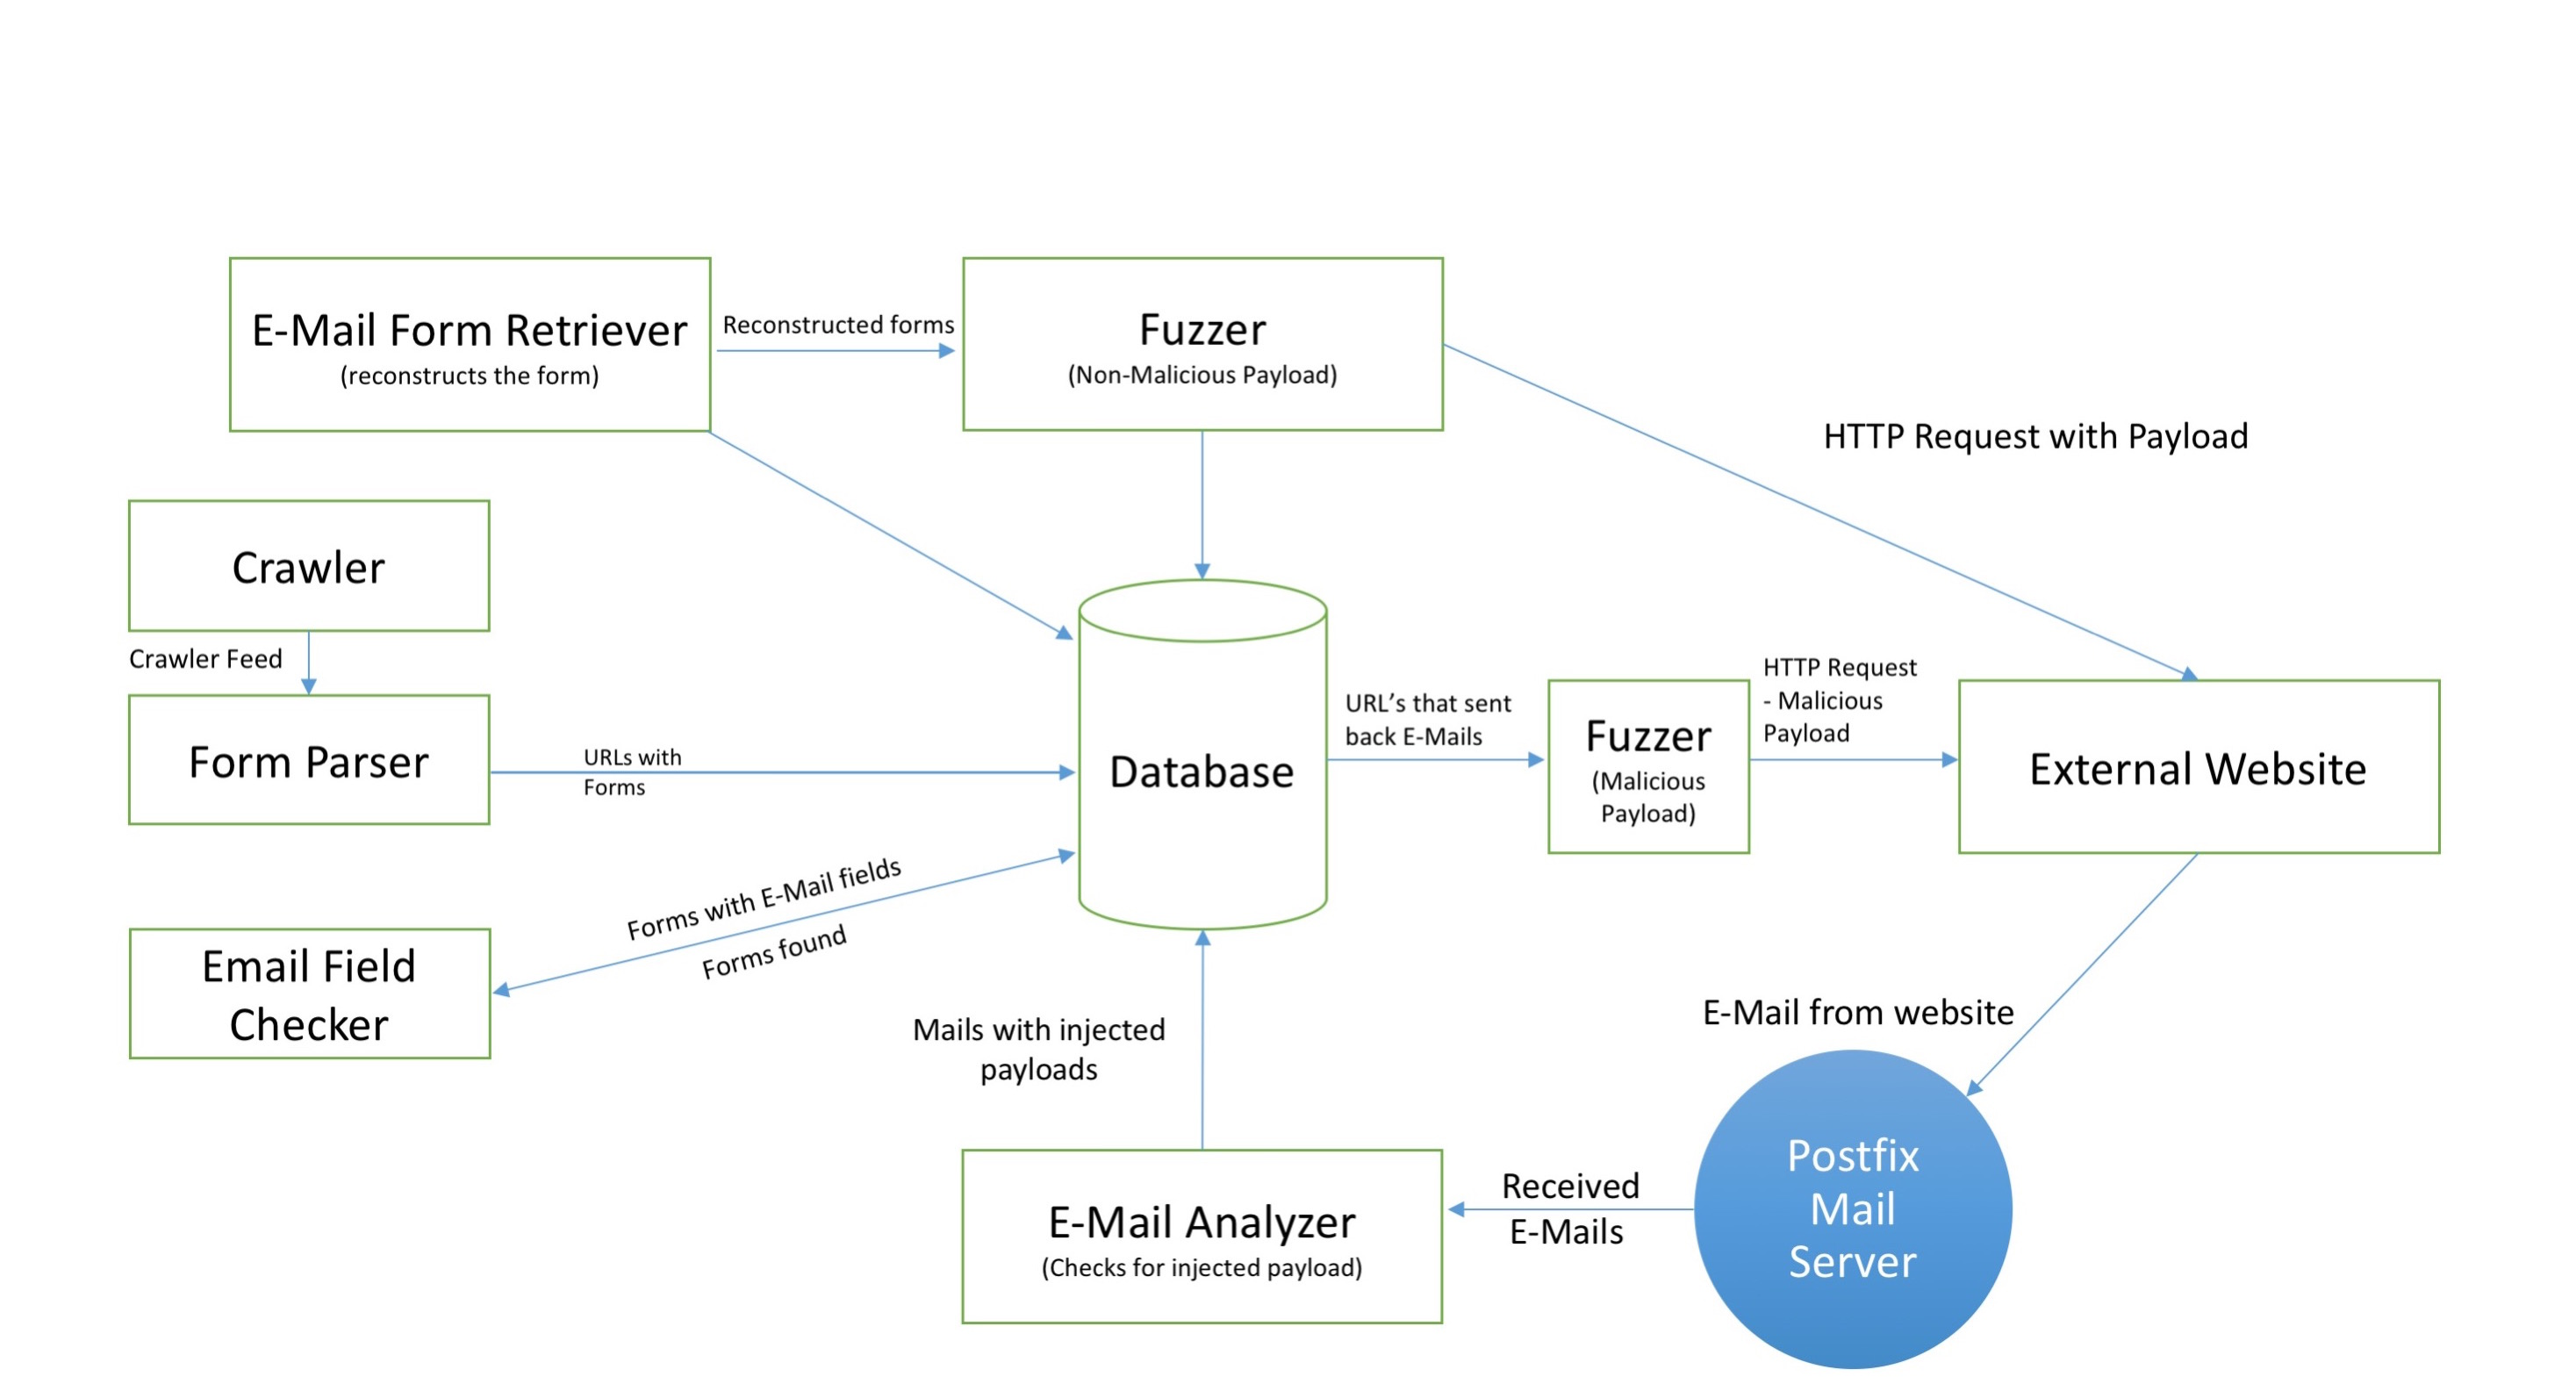
\includegraphics[width=14cm, height=7cm]{overall}
	\caption{Overall system architecture.}
	\label{fig:overall}
\end{figure*}

\subsection{System Architecture}
\label{sys:arch}
The black-box testing system can be divided broadly into two modules; Data Gathering and Payload Injection.
\begin{enumerate}
	\item Data Gathering\\
	The Data Gathering module (shown in Figure~\ref{fig:crawler}) is primarily responsible for the following activities:
	\begin{itemize}
		\item Interface with the Crawler (Section \ref{Comp:Crawler}) and receive the URLs.
		\item Parse the HTML for the corresponding URL and store the relevant form data (Section \ref{Comp:FP}).
		\item Check for the presence of forms that allow the user to send/receive e-mail, and store references to these forms (Section \ref{Comp:EMFC}).
	\end{itemize} 
	\item Payload Injection\\
	The Payload Injection module (shown in Figure~\ref{fig:fuzzer}) is primarily responsible for the following activities:
	\begin{itemize}
		\item Retrieve the forms that allow users of a website to send/receive e-mail and reconstruct these forms (Section \ref{Comp:EMFR}).
		\item Inject these forms with benign data (non-malicious payloads) and generate an HTTP request to the corresponding URL (Section \ref{Comp:Fuzzer:nmp}).
		\item Analyze the e-mails, extracting the header fields and checking for the presence of the injected payloads (Section \ref{Comp:EMA}).
		\item Inject the forms that sent us e-mails with malicious payloads, and generate an HTTP request to the corresponding URL to check if E-Mail Header Injection vulnerability exists in that form (Section \ref{Comp:Fuzzer:mp}).
	\end{itemize} 
	The functionality of each component is discussed further in the `Components' section (Section~\ref{Comp}). The Payload Injection pipeline is not a linear, but cyclic process, as we inject different payloads and analyze the received e-mails.
\end{enumerate}

\begin{figure}
	\centering
	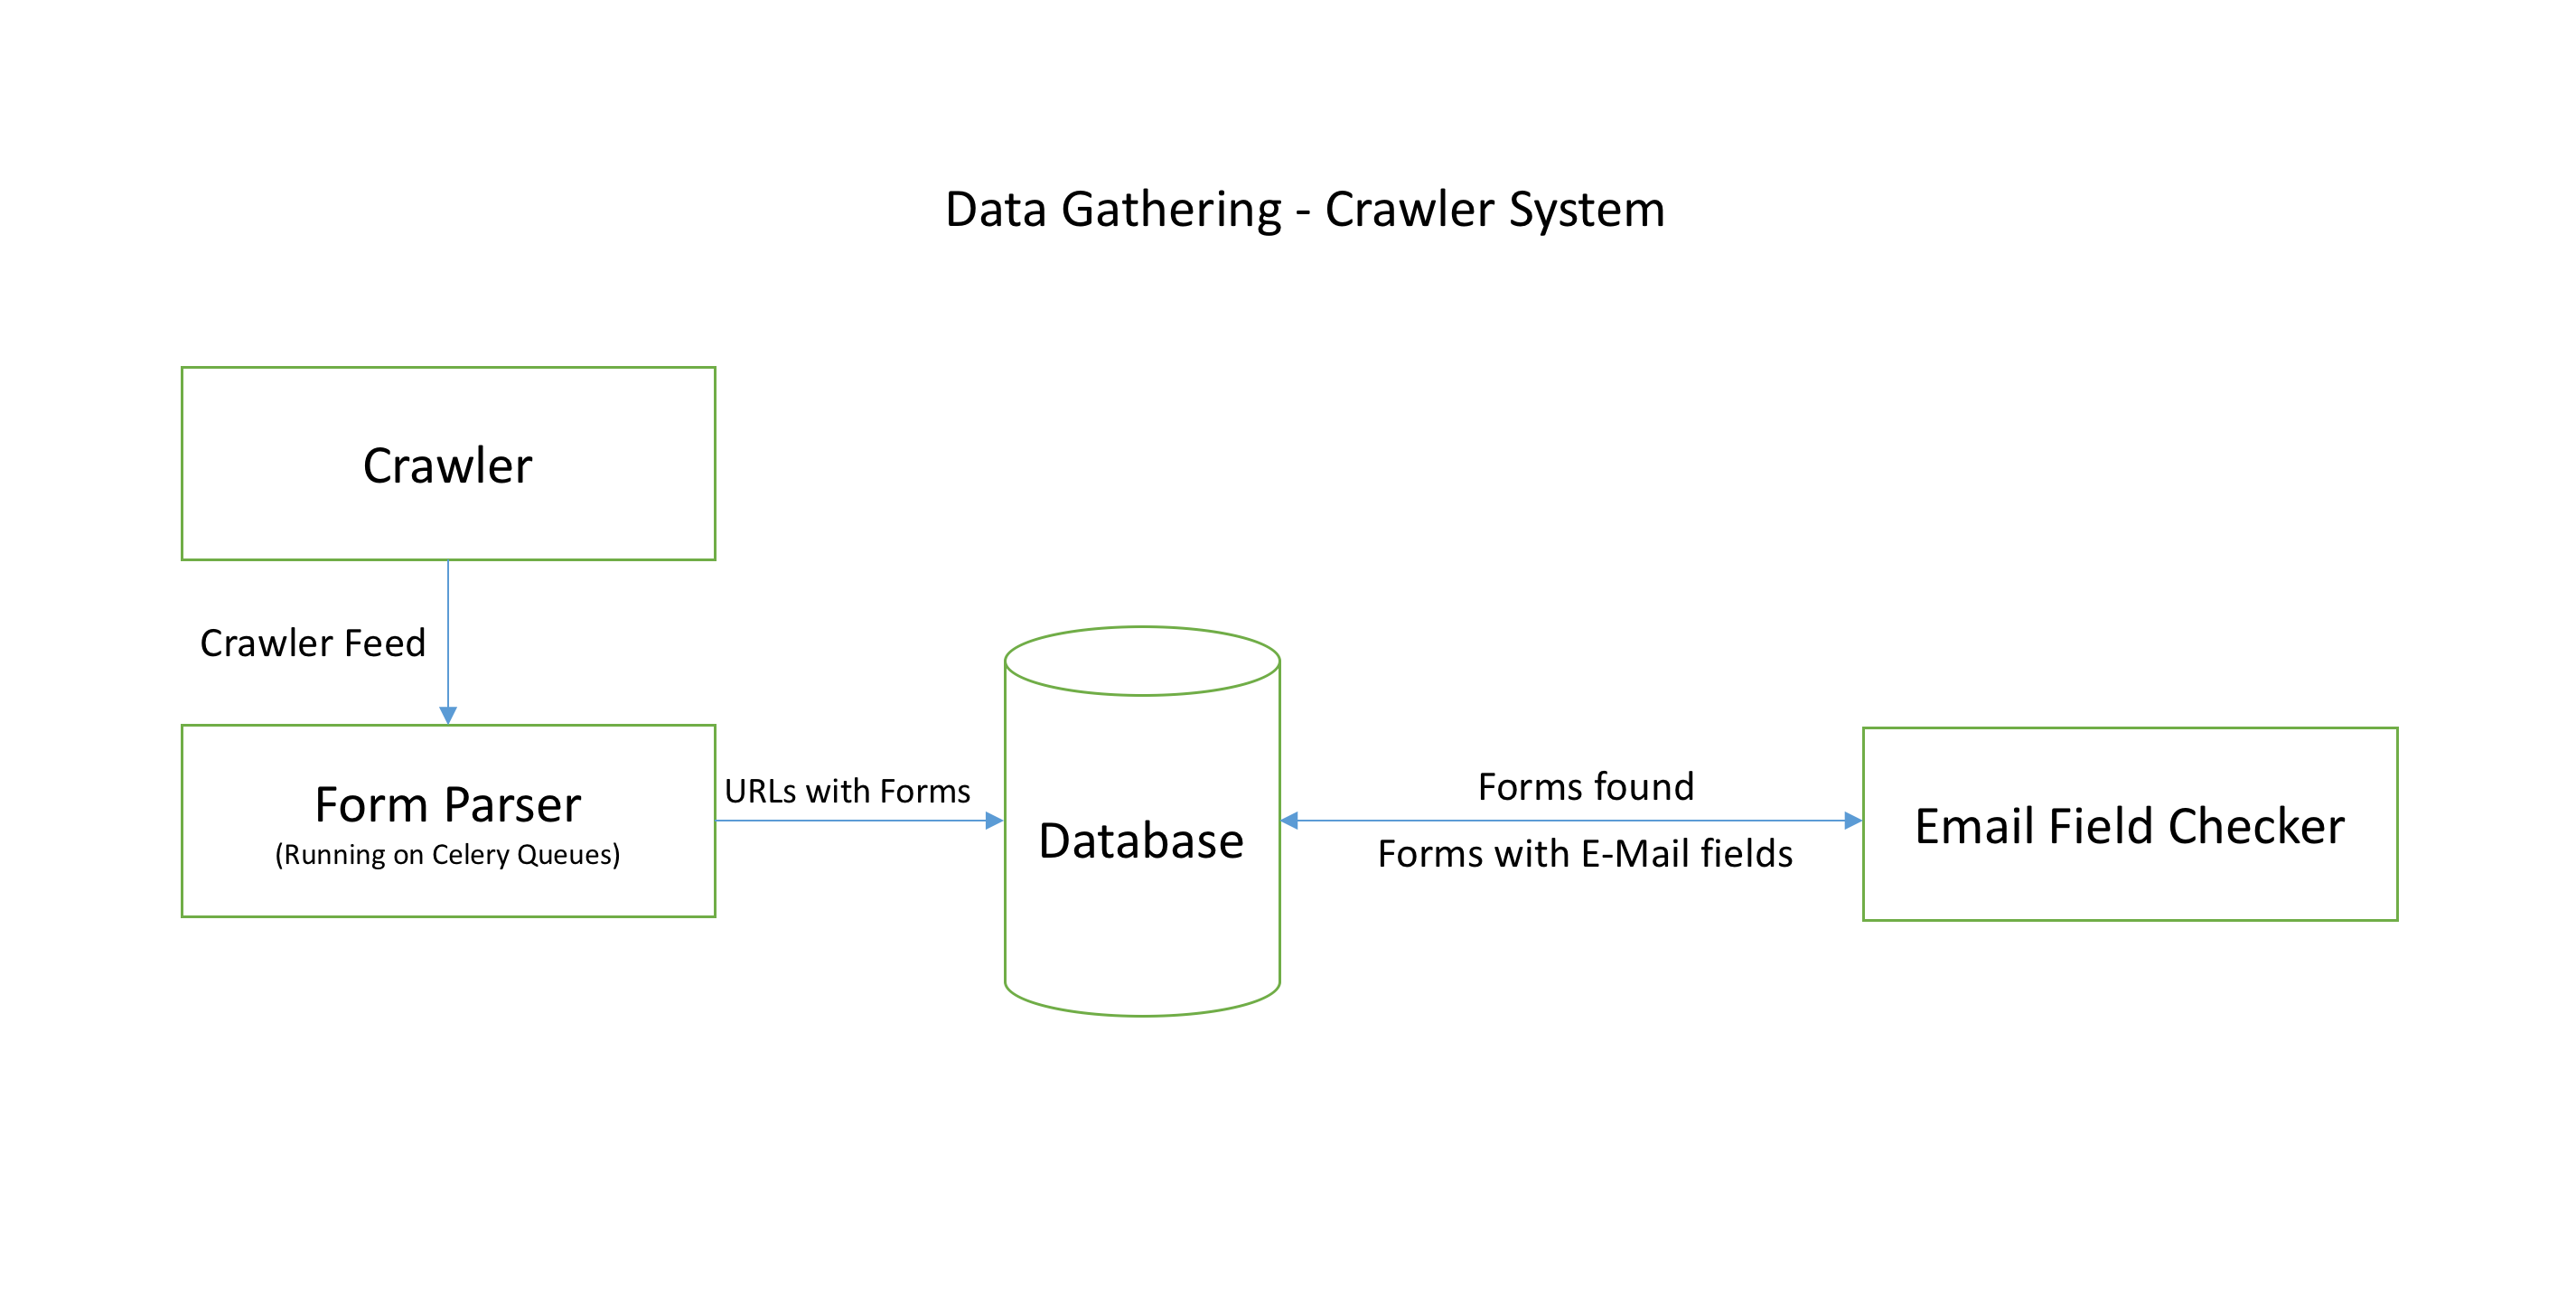
\includegraphics[width=14cm, height=7cm]{System/crawler_design}
	\caption[\titlecap{System architecture - crawler}]{System architecture - crawler \& form parser.}
	\label{fig:crawler}
\end{figure}


\begin{figure}
	\centering
	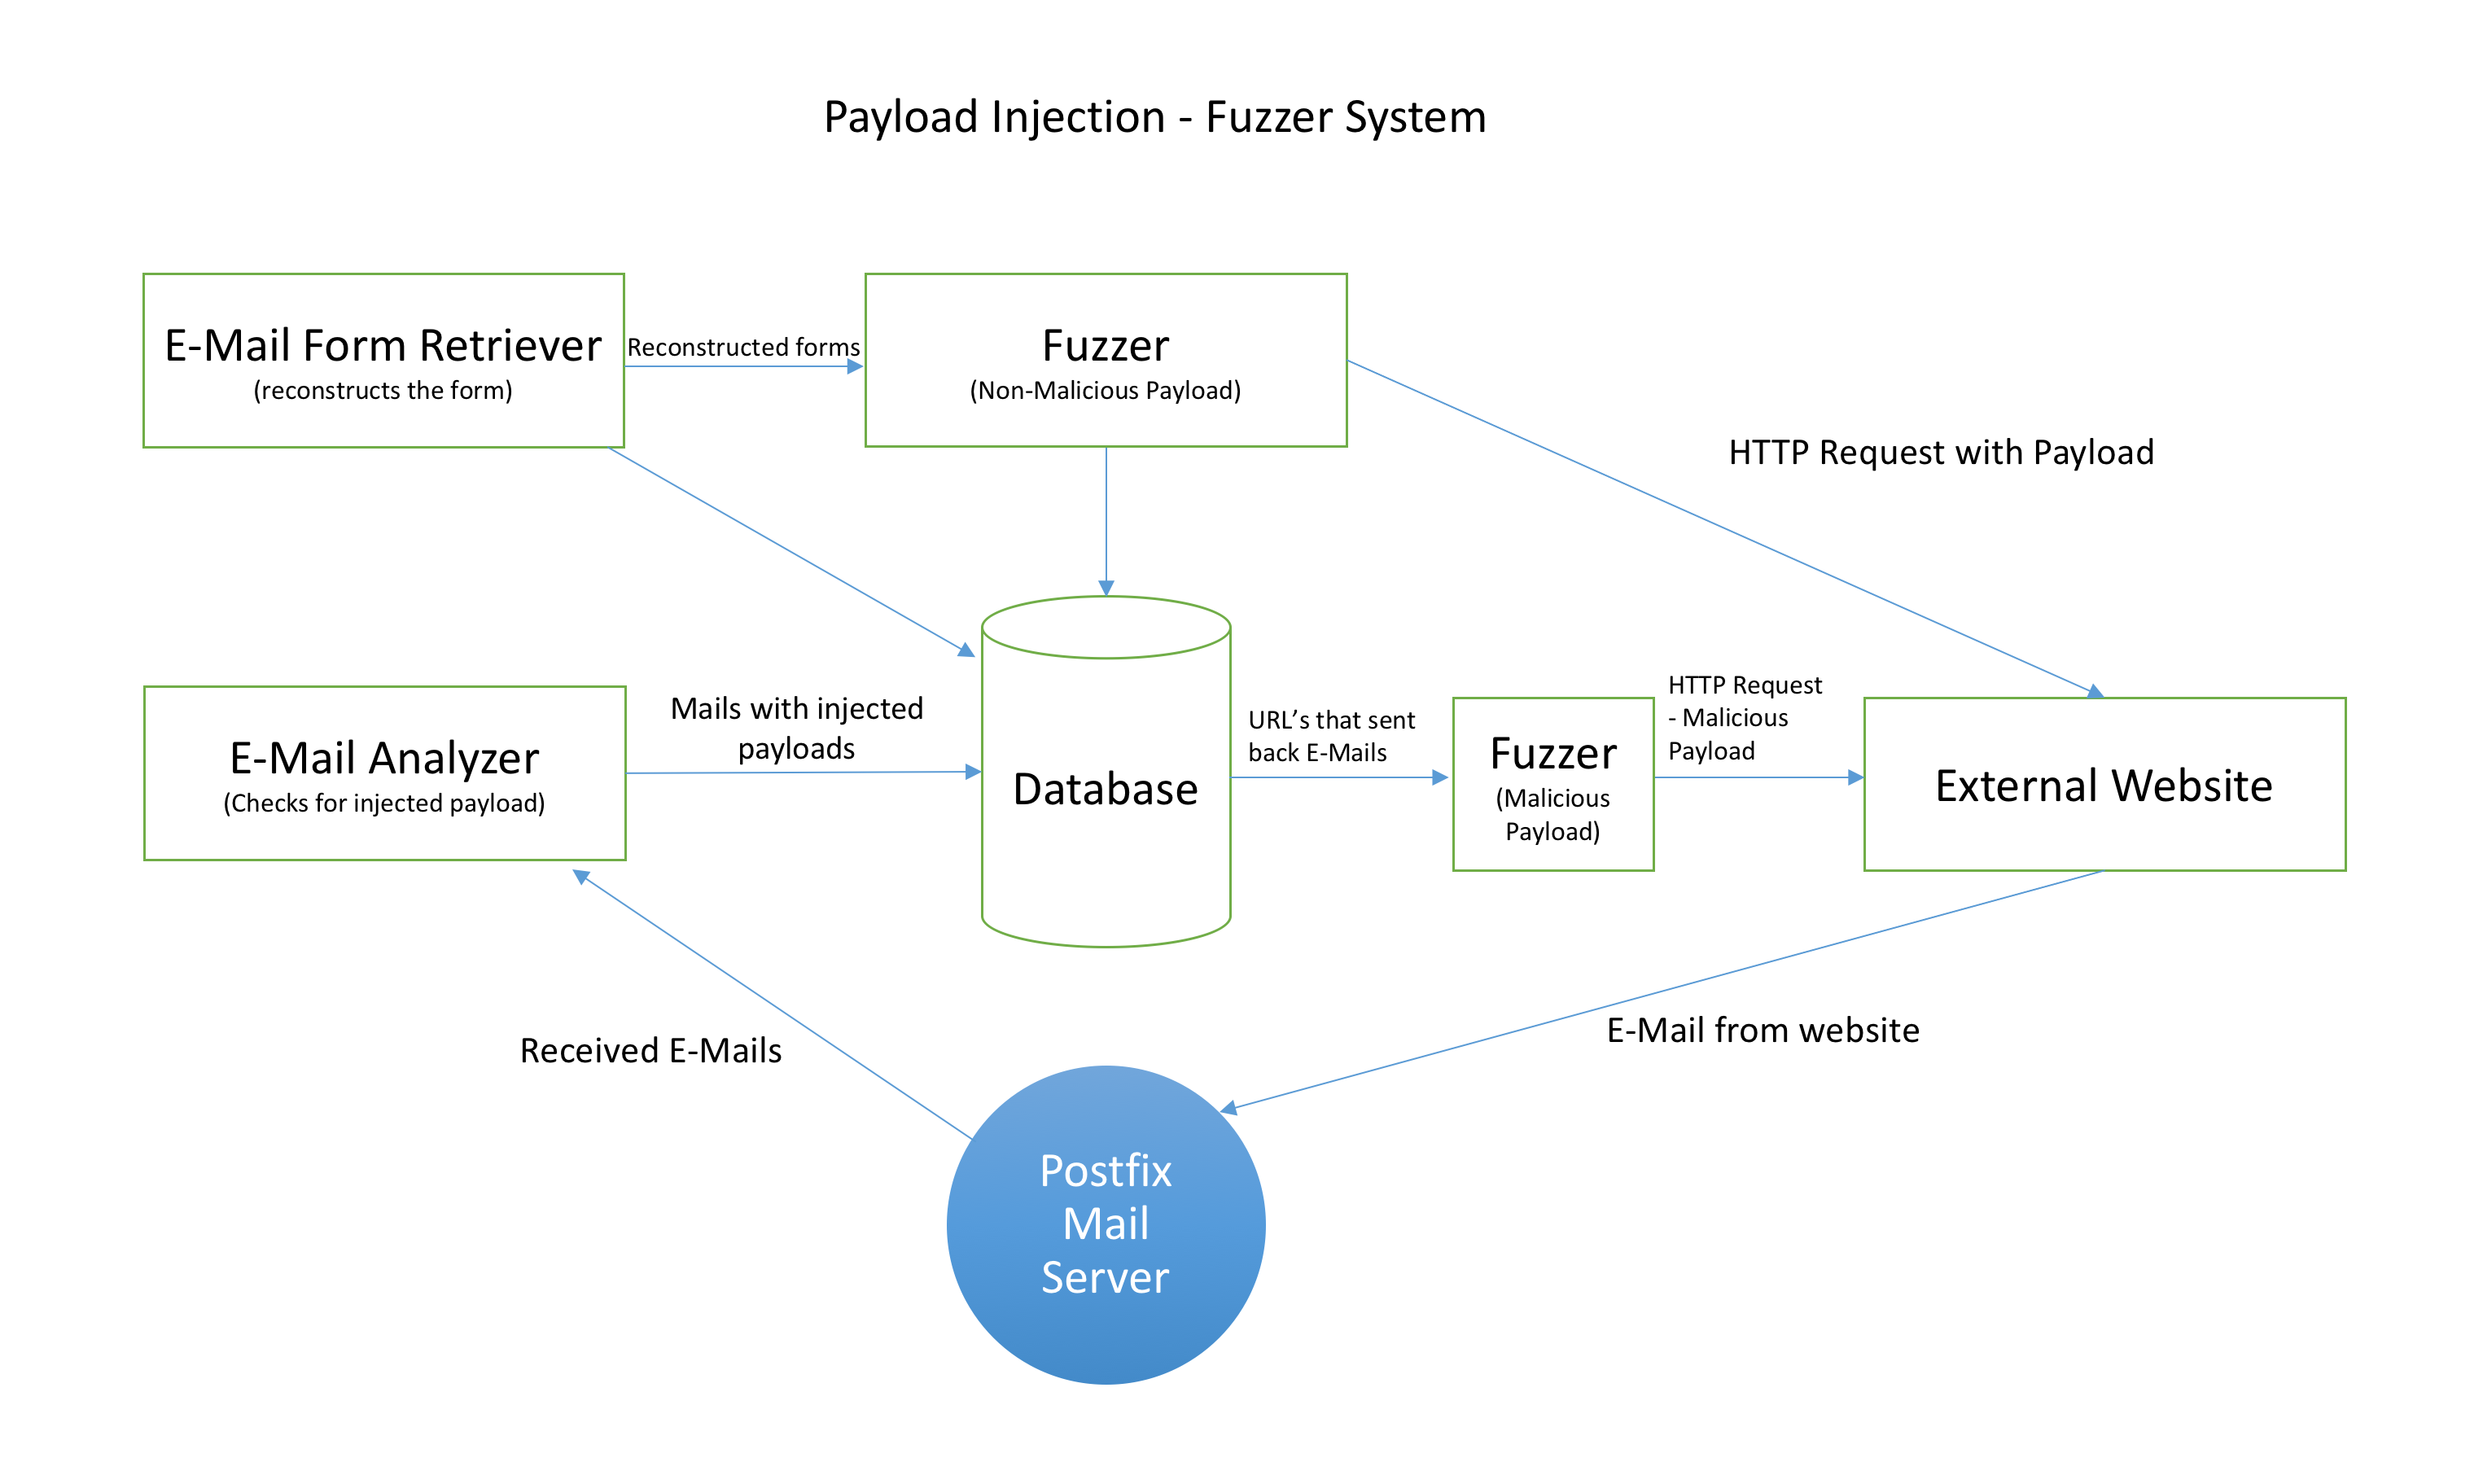
\includegraphics[width=16cm, height=9cm]{System/fuzzer_design}
	\caption[\titlecap{System architecture - fuzzer {\&} e-mail analyzer}]{System architecture - fuzzer {\&} e-mail analyzer.}
	\label{fig:fuzzer}
\end{figure}

\subsection{System Components}
\label{Comp}

The Data Gathering module and Payload Injection modules are composed of smaller components. This section describes the functionality of those components.

\subsubsection{Data Gathering}
\label{Comp:Crawler}
We used an open-source Apache Nutch based Crawler~\cite{nutch}. The \texttt{Crawler} provides the system with a continuous feed of URLs and the HTML contained in those pages. 
\label{Comp:FP}
The \texttt{Form Parser} is responsible for parsing the HTML and retrieving data about the HTML
forms on the page, including the following: (1) Form attributes, such
as \texttt{method} and \texttt{action} (URL) for the HTTP request, (2)
Data about the form input fields, such as their attributes, names, and
default values. The default values are essential for fields like
{\lstinline{<input type="hidden">}} as these fields are usually used
to check for the submission of forms by bots, and (3) Presence of the {\lstinline{<base>}} element in the HTML, as this affects the final URL to which the form is to be submitted (if the \texttt{action} attribute is a relative URL).

\label{Comp:EMFC}
The \texttt{\Email Field Checker} is the final stage in the Data Gathering module. It receives the HTML form data and checks for the presence of \email fields in those forms. If any \email fields are found, it stores references to these forms.
The intuition here is that we do not want to try to fuzz all HTML forms on the web to look for \ehi vulnerabilities, rather just those HTML forms that are likely to invoke server-side email functionality.

The \Email Field Checker searches for the words \texttt{e-mail},
\texttt{mail} or \texttt{email} within the form, instead of an
explicit HTML5 \email field (e.g.,\ {\lstinline{<input type="email">}}). This is by design, taking into account a common
design pattern used by web developers, where they may have a text
field with an \texttt{id} or \texttt{name} attribute set to
\texttt{email}, instead of an actual \email type attribute, for
purposes of backward compatibility with older browsers. The output of this stage is stored in the database for persistence and acts as the input to the Payload Injection module.

%% Compared to searching for explicit \email fields, by searching for the presence of the words \texttt{\email}, \texttt{mail} or \texttt{email} in the form, we are assured very few false negatives. This is because our system is bound to find \email fields with their \texttt{type}, \texttt{name}, or \texttt{id} set to one of these words. The system is also substantially faster as we do not have to parse the individual form fields at this point in the pipeline. However, despite the advantages, this might also lead to a false positive rate. We discuss this possibility in detail in Section~\ref*{issues:fpr} - Design Issues.


\subsubsection{\Email Form Retriever}
\label{Comp:EMFR}
The \Email Form Retriever is the first stage in the Payload Injection
module. It has the following functions: (1) Retrieve new forms and
ensure no duplication occurs before the fuzzing stage, (2) reconstruct
each form, using the stored form data, specifically the input fields
and their values, and (3) construct the target URL for the
\texttt{action} attribute of the form to create an HTTP request to the
correct URL for fuzzing.


\subsubsection{Fuzzer}
\label{Comp:Fuzzer}
% Adam: we should call these something else but modules. We already have the top two modules, which are composed of components, now we need to split these into something (not components again). - DONE
The Fuzzer is the only component that interacts directly with the external web applications. The Fuzzer is split into smaller parts, each of which is responsible for a particular type of fuzzing.  The system injects payloads in two stages: the goal is to reduce the total number of HTTP requests the system generates to detect an \ehi vulnerability. Making HTTP requests is an expensive process~\cite{httpperf}, and can cause bottlenecks in a Crawler-Fuzzer system~\cite{ShkapenyukTorstenSuel2001}.
The two different types of payloads used for fuzzing are:

\noindent\textbf{Non-Malicious Payload.}
The regular or non-malicious payload is simply an \email address. The goal is to see if the web application will send an \email message based on our input. The specific format of the \email is \lstinline|reguser(xxxx)@example.com|, where \texttt{xxxx} is replaced by an internal id that uniquely maps the payload to the form, and \texttt{example.com} is replaced by our domain.

\noindent\textbf{Malicious Payload.}
After receiving an \email from a specific form, we then use the malicious payload to try to exploit an \ehi vulnerability. We inject the form parameters with the \texttt{bcc} (blind carbon copy) header. If the vulnerability is present, this will cause the server to send a copy of the \email to the \email address we added as the \texttt{bcc} field.

We consider a special case: the addition of an \texttt{x-check:in} header field to the payloads. This is due to Python's exhibited behavior when attaching
headers. Instead of overwriting a header if it is already present, Python will ignore duplicate headers. So, if the \texttt{bcc} field is already present as part of the headers, our injected \texttt{bcc} header would be ignored. To overcome this, we inject a new header that is not likely to be generated by the web application. 

We created four different malicious payloads. Each of these payloads
is crafted for a particular use case. The four payloads are:
(1) nuser(xxxx)@example.com\textbackslash{}n\-bcc:\-maluser\-(xxxx)\-@example.com,
(2) nuser(xxxx)@\-example.com\textbackslash{}n\-bcc:\-maluser\-(xxxx)\-@example.com\textbackslash{}n\-x-check:in,
(3) nuser(xxxx)@\-example.com\textbackslash{}r\textbackslash{}n\-bcc:\-maluser(xxxx)\-@example.com,
and (4) nuser(xxxx)\-@example.com\textbackslash{}r\textbackslash{}n\-bcc:\-maluser(xxxx)\-@example.\-com\textbackslash{}r\textbackslash{}n\-x-check:in.
	
Payload 1 is the most minimal payload: it injects a newline character followed by the \texttt{bcc} field. Payload 2 contains the additional \texttt{x-check} header to inject Python-based web applications. Payloads 3 and 4 are added for purposes of cross-platform fuzzing: \texttt{\textbackslash{}r\textbackslash{}n} is the ``Carriage Return - New Line (CRLF)'' used on Windows systems.~\cite{rfc2616}

The \texttt{(xxxx)} in each payload is replaced by an internal unique id to create a one-to-one mapping of the payloads to the forms.
% Adam: If we need to cut things for space, we can cut this next line and the payload coverage table.

%\begin{table}[tbp]
%	\centering
%	\normalsize
%	\begin{tabular}{|c|c|c|}
%		\hline
%		\multicolumn{1}{|c|}{\textbf{Payload}} & \multicolumn{1}{c}{\textbf{Languages covered}} & \multicolumn{1}{|c|}{\textbf{Platforms covered}}\\
%		\hline
%		1 & PHP, Java, Ruby, etc. & Unix\\
%		\hline
%		2 & PHP, Java, Ruby, etc. & Windows\\
%		\hline
%		3 & Python & Unix\\
%		\hline
%		4 & Python & Windows\\
%		\hline
%	\end{tabular}
%	\caption[\titlecap{Payload coverage}]{Payload coverage, each payload covers a different platform/language.}
%	\label{tab:payloadcov}
%\end{table}

%% \begin{table}[tbp]
%% 	\centering
%% 	\scriptsize
%% 	\begin{tabular}{|c|c|c|}
%% 		\hline
%% 		\multicolumn{1}{|c|}{\textbf{Language/Platform}} & \multicolumn{1}{c}{\textbf{Unix}} & \multicolumn{1}{|c|}{\textbf{Windows}}\\
%% 		\hline
%% 		\textbf{PHP, Java, Ruby} & 1 & 3\\
%% 		\hline
%% 		\textbf{Python} & 2 & 4\\
%% 		\hline
%% 	\end{tabular}
%% 	\caption[\titlecap{Payload coverage}]{Payload coverage, each payload covers a different platform/language.}
%% 	\label{tab:payloadcov}
%% \end{table}

Along with the payload, the Fuzzer also injects data into the other fields of the form. This data must pass validation constraints on the individual input fields (e.g.,\ for a name field, numbers might not be allowed).  As crawling and fuzzing input fields on the web is an open problem~\cite{raghavan2000crawling}, we chose to go with a best-effort approach. To maximize the amount of vulnerabilities the system discovers, the data injected into the input fields should adhere to the constraints. The Fuzzer uses a ``Data Dictionary'' which has predefined ``keys'' and ``values'' for standard input fields such as \texttt{name}, \texttt{date}, \texttt{username}, \texttt{password}, \texttt{text}, and \texttt{submit}.
% Adam: What does it mean here for these to be generated on-the-fly? Using templates? - Fixed.
The values for these are generated from the Data dictionary for each form, based on generally followed guidelines for such fields. For example, password fields should consist of at least one uppercase letter, one lowercase letter, and special characters.
% Adam: can you add a sentence here about crawling and fuzzing fields on the web is an open problem (and cite ``Crawling the hidden web'' - DONE.

When the fuzzed data is ready, the Fuzzer constructs the appropriate HTTP request (GET or POST) and sends the HTTP request to the URL that was generated by the \Email Form Retriever (Section~\ref{Comp:EMFR}). 


\subsubsection{Injection Verification}
\label{Comp:EMA}
The Injection Verification module checks for the presence of injected data in the received \emails. This module works on the \emails received and stored by our Postfix server, and, depending on the user account that received the \email, it performs different functions.

\noindent\textbf{Analyzing regular e-mail.}
\sloppy
`Regular \email' refers to the \emails received by account {\lstinline{reguser(xxxx)@example.com}} that were sent due to injecting the regular, non-malicious, payload (discussed in Section~\ref{Comp:Fuzzer}). The objective of the analysis on this \email is identify if the input fields that we injected with data appear on the resulting \email, and if so, which fields appear where.

%TODO Adam: made clear that ALL input fields that appear in the email are fuzzed, with examples like name, username, etc.
To find this, we parse each received \email, and check whether \emph{any} of the fields we injected with data appear as part of either the headers or the body of the \email. These could be fields such as name, date of birth, username, etc. If they do, we add them to the list of fields that can \emph{potentially} result in an \ehi vulnerability for the given \email. 

We then pass on this information back to the Fuzzer pipeline, along with the vulnerable form, where these fields are \emph{also} fuzzed along with the \email fields to check for the presence of \ehi.

\noindent\textbf{Analyzing \email with payloads}
The ``\emails with payloads'' refers to \emails received by either the {\lstinline{nuser(xxxx)@example.com}} or {\lstinline{maluser(xxxx)@example.com}} accounts. These \emails could only be received as a result of injecting the malicious payloads that were discussed in Section~\ref{Comp:Fuzzer}. 

\noindent\textbf{Detecting injected \texttt{bcc} headers}
As discussed in the payloads Section~(\ref{Comp:Fuzzer}), the payloads were crafted such that the \emails received by the \texttt{maluser} account directly indicate the presence of the injected \texttt{bcc} field. 

\label{analyze:detect_x_check}
\noindent\textbf{Detecting injected \texttt{x-check} headers} \Emails
not received by the \texttt{maluser} account but by the \texttt{nuser}
account constitute a special category of \emails. These \emails could
have been generated due to two reasons: (1) The web application
performed some sanitization routines and stripped out the \texttt{bcc}
part of the payload, thereby sending \emails only to the
\texttt{nuser} account. These \emails then act as proof that the
vulnerability was not found on the given URL. (2) The \texttt{bcc}
header can be ignored for other reasons (e.g.,\ Python's default
behavior when it encounters duplicate headers). In this case, we check
if the \email contains the custom header \texttt{x-check}. If it does,
then this is a successful exploit of the vulnerability.

%\section{Test Suite}
\label{Arch:Test}
The test plan for our system includes a set of unit tests for each module in the pipeline. Further, we have unit tests for every %every instead of each
individual function in the modules. The functions are tested separately, using mocks and stubs, so as to ensure isolated testing.
This section outlines the test plan in the following manner. We list the modules that are tested, and then describe what each unit test tests for.
\begin{itemize}
	\item Form Parser
	\begin{itemize}
		\item \colorbox{lightgray}{\lstinline{test_url_exception}} - Tests whether the system handles incorrect or malformed URLs properly and terminates cleanly.
		\item \colorbox{lightgray}{\lstinline{test_db_connection}} - Tests whether the Database Connection is set up and queries can be executed.
		\item \colorbox{lightgray}{\lstinline{test_form_parser}} - Tests for the proper parsing of HTML, and if the system exits cleanly in case parsing is not possible.
	\end{itemize}
	
	\item E-Mail Field Checker
	\begin{itemize}
		\item \colorbox{lightgray}{\lstinline{test_check_for_email}} - Tests whether the system finds E-Mail fields in the form when the words `e-mail' or `email' are present in the form (case insensitive).
		\item \colorbox{lightgray}{\lstinline{test_check_for_no_email}} - Tests whether the system finds no E-Mail fields when the words `e-mail' or `email' are \emph{not} present in the form (case insensitive).
	\end{itemize}
	
	\item E-Mail Form Retriever
	\begin{itemize}
		\item \colorbox{lightgray}{\lstinline{test_reconstruct_form}} - Tests for the proper reconstruction of the form stored in the Database.
		\item \colorbox{lightgray}{\lstinline{test_construct_url}} - Tests whether the URL for submission was constructed properly, includes checks for relative URLs, absolute URLs, and presence of \lstinline{`base'} tags.
		\item \colorbox{lightgray}{\lstinline{test_email_form_retriever_already_fuzzed}} - Tests for duplicate fuzz requests, and whether the system rejects these requests.
		\item \colorbox{lightgray}{\lstinline{test_email_form_retriever_calls_fuzzer_for_new_fuzz}} - Tests whether the E-Mail Form Retriever calls the Fuzzer module with the proper data when it gets a new fuzz request.
	\end{itemize}
	
	\item Fuzzer
	\begin{itemize}
		\item \colorbox{lightgray}{\lstinline{test_send_get_request}} - Tests for the proper handling of GET requests.
		\item \colorbox{lightgray}{\lstinline{test_send_post_request}} - Tests for the proper handling of POST requests.
		\item \colorbox{lightgray}{\lstinline{test_correct_fuzzer_data}} - Tests whether the payload generated for the given form data is correct and consistent. Also tests whether the payload was part of the resulting HTTP request.
		\item \colorbox{lightgray}{\lstinline{test_incorrect_fuzzer_data}} - Tests for incorrect form data, and ensures that a payload does not end up in the wrong input field in the resulting HTTP request.
	\end{itemize}
	\item E-Mail Analyzer
	\begin{itemize}
		\item \colorbox{lightgray}{\lstinline{test_load_mail}} - Tests whether the E-Mails are loaded and parsed correctly by the E-Mail Analyzer.
		\item \colorbox{lightgray}{\lstinline{test_parse_headers}} - Tests for the proper parsing of headers present in the E-Mail.
		\item \colorbox{lightgray}{\lstinline{test_analyze_regular_mail}} - Tests whether the E-Mail Analyzer parses the regular E-Mail properly and extracts the injected input fields that are present in the E-Mail.
		\item \colorbox{lightgray}{\lstinline{test_analyze_malicious_mail}} - Tests whether the E-Mail Analyzer parses the E-Mails received due to the malicious payloads properly, is able to extract the `bcc' headers, and is able to link them to the proper fuzzing request and payload.
		\item \colorbox{lightgray}{\lstinline{test_analyze_x_check_header}} - Tests whether the `x-check' header is read by the E-Mail Analyzer.
	\end{itemize}
\end{itemize}
The unit tests were written using Python's built-in `Unittest' module, mocking was done using the built-in `MagicMock' module. The tests allow us to be reasonably certain that our system works as expected.

%\subsection*{Proof of Concept Attacks}
This section describes how we validated our expectations. In order to do this, we constructed three sets of web applications in PHP, Python, and Ruby. Each of these applications was a simple web app that accepted user input to construct and send an E-Mail.

The front-end for each of the three applications is shown in Listing~\ref{code:html}. The server-side code for the PHP and Python are shown in Listings~\ref{code:phpemi} and \ref{code:pyemi} respectively.

We tested for the headers being injected in real-time by running an instance of MailCatcher, set to listen on all SMTP messages. A sample screenshot of a fuzzed request for the Ruby backend (generated in PostMan) is shown in Figure~\ref{fig:postmanruby}. The e-mail sent due to injecting this payload (as captured by MailCatcher) is shown in Figure~\ref{fig:mailcatcherruby}. It can be seen that the headers have been added to the resulting e-mail, and we have successfully managed to overwrite the \texttt{Subject} field with our message, `hello'.

The astute reader might have noticed that in the given example we have used \texttt{\%0a} to separate the headers, while in Section~\ref{Comp:Fuzzer:mp}, we had used \texttt{\textbackslash{}n}. This is due to URL encoding~\cite{rfc1738}, wherein special characters in th URL are `encoded' or `escaped' with their ASCII equivalent.
The reason why we do not have to do this with the payloads our system injects is due to the fact that the Python Requests library that we use to generate the HTTP requests automatically does this encoding for us.

\lstset{language=HTML,caption={HTML page for showcasing e-mail header injection, a simple front-end for our examples.},label={code:html}}
\begin{lstlisting}
<!doctype html>
<html lang="en">
<head>
<meta charset="utf-8">
<meta name="author" content="Sai Pc">
<title>Mock Email</title>
</head>
<body>
<form action="{Replace with path to back-end}" method="post">
<input type="text" placeholder="Email" name="email" id="e-mail"><br>
<textarea name="msg" rows="20" cols="120"></textarea>
<input type="submit" value="Email Me!">
</form>
</body>
</html>
\end{lstlisting}

\begin{figure}[!htbp]
	\centering
	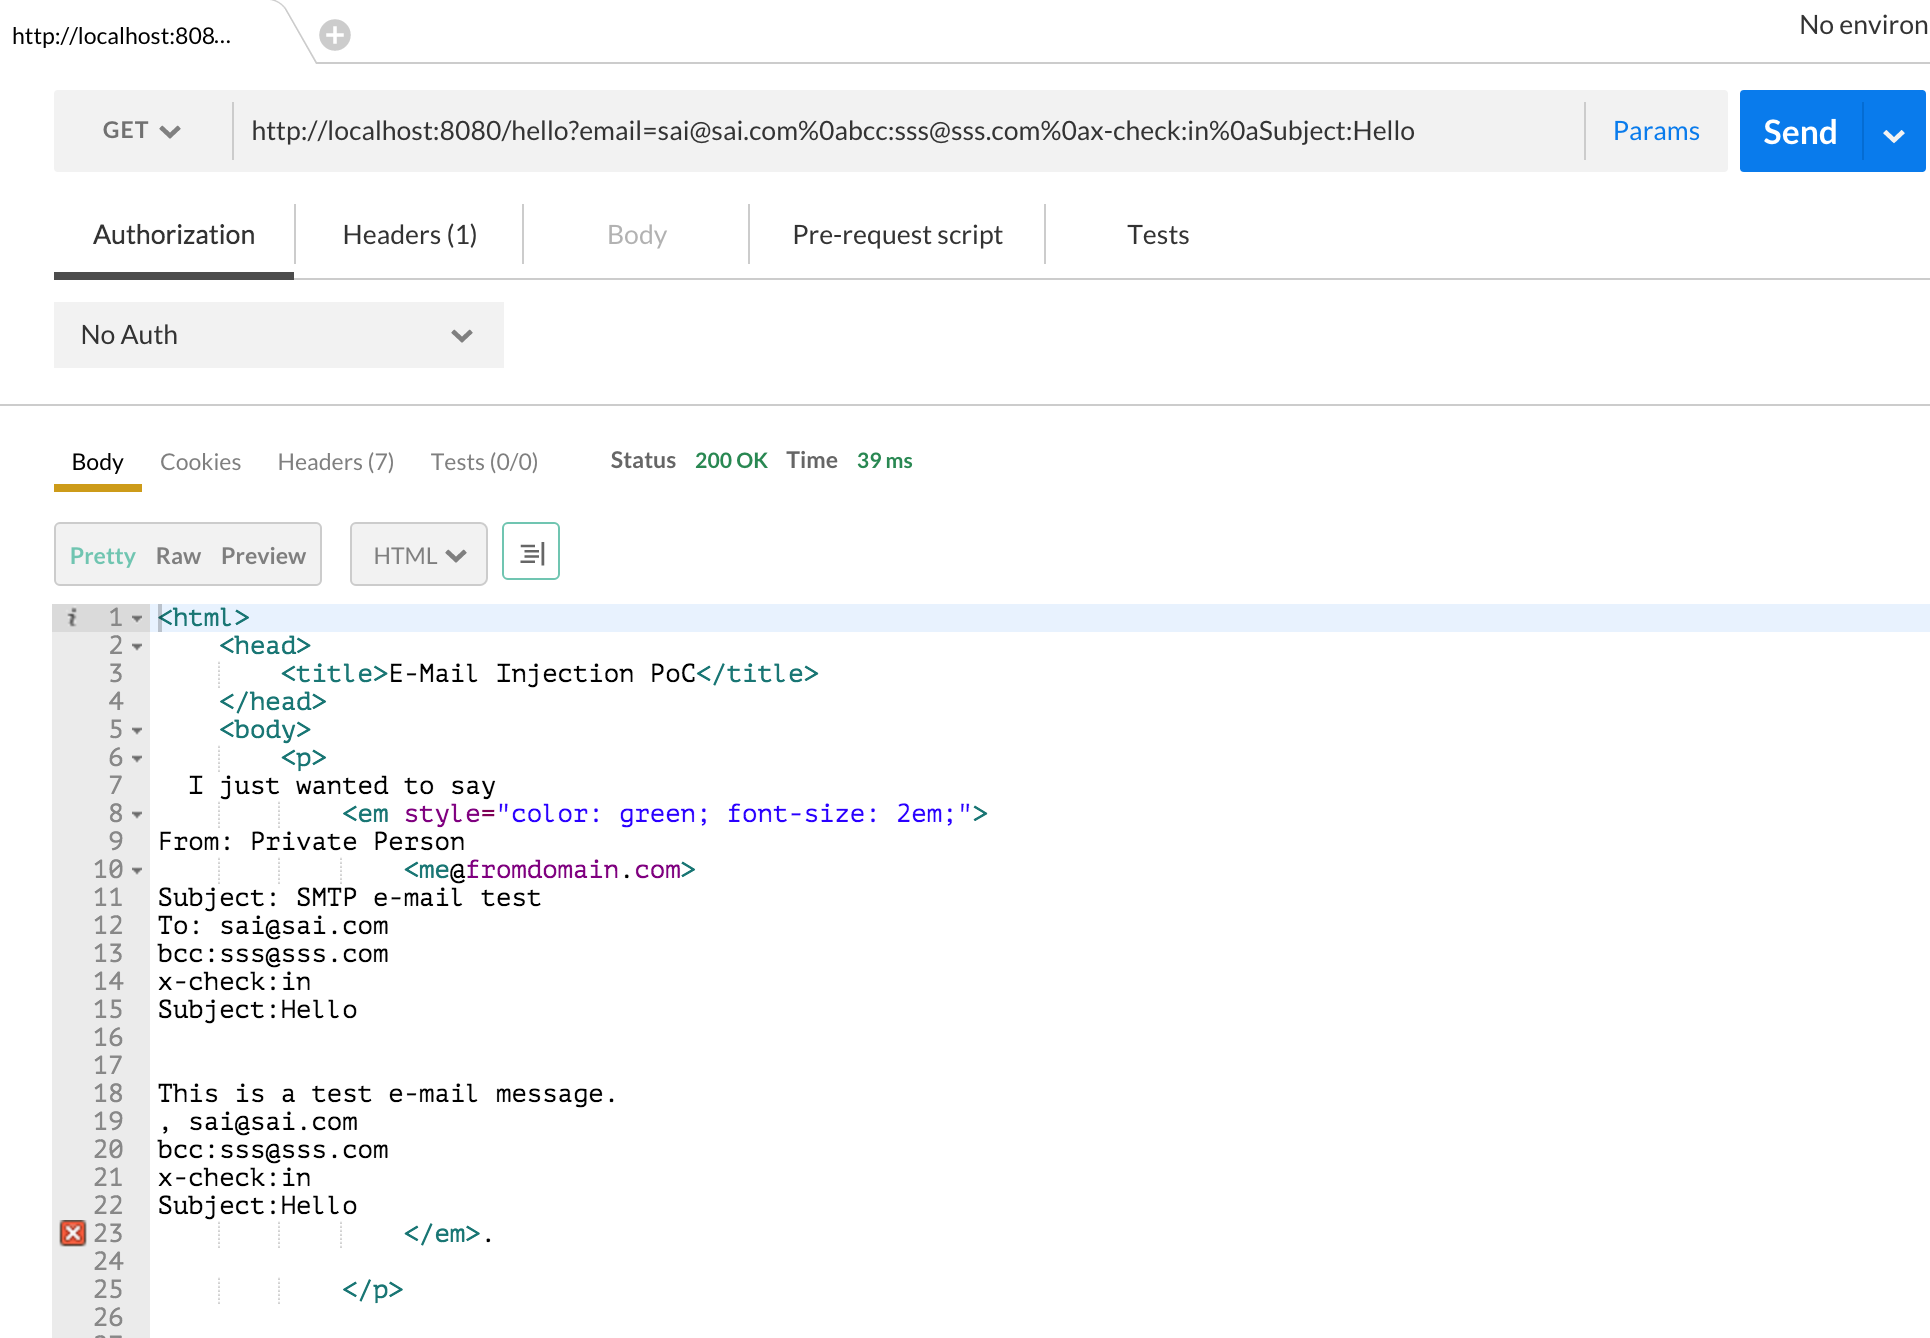
\includegraphics[width=14cm, height=8cm]{System/EMI_Postman_Ruby}
	\caption[\titlecap{Fuzzing a request for the Ruby backend}]{Fuzzing a request for the Ruby backend, the payload can be seen inside the address bar.}
	\label{fig:postmanruby}
\end{figure}

\begin{figure}[!htbp]
	\centering
	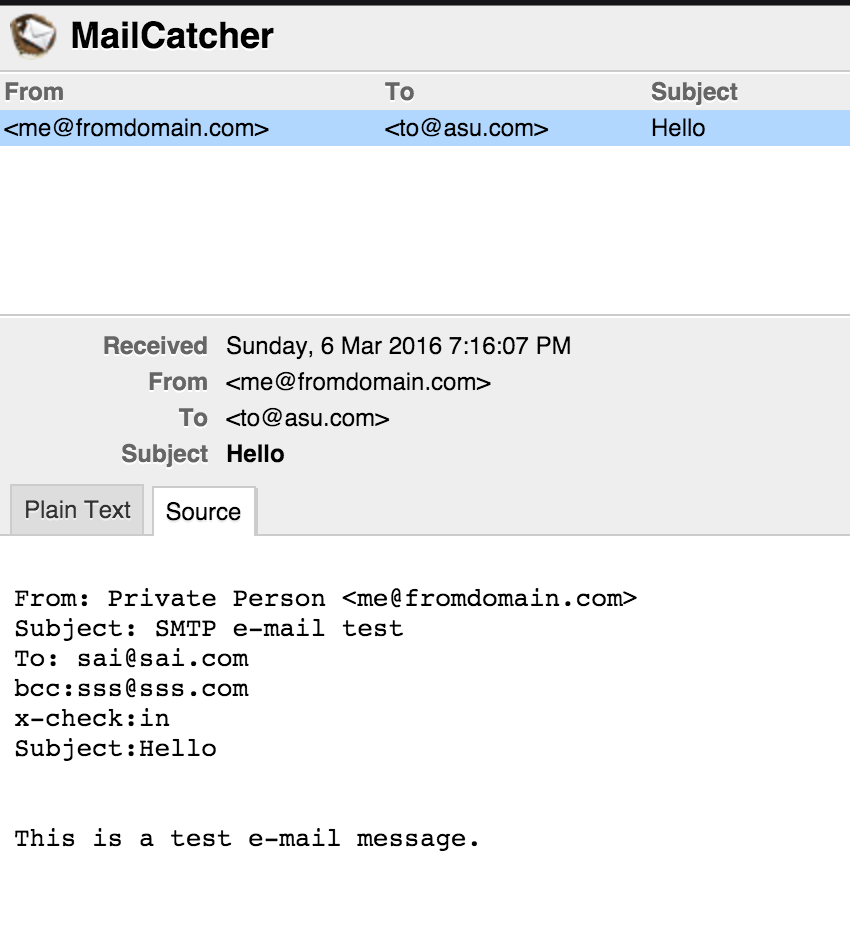
\includegraphics[width=14cm, height=8cm]{System/EMI_Mailcatcher_Ruby}
	\caption[\titlecap{E-Mail header injection proof of concept - Ruby}]{E-Mail header injection proof of concept - Ruby, we can see that multiple headers (bcc, x-check, subject) have been inserted into the resulting e-mail.}
	\label{fig:mailcatcherruby}
\end{figure}
\section[Issues]{Design Issues}
\label{sys:issues}
This section will describe the issues we faced with the design decisions we made, and how we did our best to mitigate them, and their effect on the system.

\begin{itemize}
	\item \label{issues:fpr}False Positive rate for the E-Mail Field Checker\\
	As discussed in Section \ref{Comp:EMFC}, we only search for the words `email', `mail' or `e-mail' (case insensitive) inside the forms to detect the presence of e-mail fields, instead of searching for an \colorbox{lightgray}{\lstinline{<input type = email>}}. This might result in a false positive in certain forms, like the one shown in Listing. \ref{code:false_positive}.
	
	\lstset{language=HTML,caption={E-Mail field checker - false positives, the system\\incorrectly classifies this as an e-mail form.},label={code:false_positive}}
	\begin{lstlisting}
	<form method="post">
	E-Mail us if you have any questions!!
	<input type="text" name="query"><br>
	<input type="submit" value="Search">
	</form>
	\end{lstlisting}
	
	The word `E-Mail' on Line 2 will result in our system classifying this form as a potential e-mail form, while it clearly is not. However, as we will see, this is not really a significant issue, as despite being added to the \lstinline{`email_forms'} table, this form will never be injected in the `fuzzer' due to the absence of the appropriate input field in the form. We chose to go with this design, as it allows us to detect almost every form that provides the capability to send or receive e-mail.
	
	\item Parallelism for the system\\
	\label{issues:parallel}
	Every component in the pipeline benefits hugely from parallel processing of the data. However, Python's GIL (Global Interpreter Lock) does not allow the running of multiple native threads concurrently. To overcome this, we used a Celery task queue (discussed in Section \ref{exp:Celery}), which allowed a level of parallelism that Python does not provide by default. Even though this makes the system faster than a single-threaded approach, it still leaves room for improvement in terms of performance. Despite the speed drop that results from lack of full parallelism, we chose to go with Python, for the raw power it provides, its text processing capabilities, PCRE (Perl Compatible Regular Expressions) compatibility, and the numerous libraries available for parsing HTML, interfacing with databases and generating HTTP requests.
	
	\item URL Construction\\
	The multiple ways in which a URL is specified (i.e.\ Relative and Absolute URLs) complicates the construction of the URL from the `action' attribute of the form.  As an example, the following URLs are all equivalent (as parsed by a browser, assuming we are in the path `www.website.com'):
	
	\begin{itemize}
		\item \colorbox{lightgray}{\lstinline{action=mail.php}}
		\item \colorbox{lightgray}{\lstinline{action=./mail.php}}
		\item \colorbox{lightgray}{\lstinline{action=http://website.com/mail.php}}
		\item \colorbox{lightgray}{\lstinline{action=www.website.com/mail.php}}
	\end{itemize}
	Add to this, if the form is a self-referencing form\,\footnotemark, and is present in mail.php, the following are equivalent to the above URLs as well:
	\footnotetext{A self-referencing form is one which submits the form data to itself. It includes logic to both display the form and process it. It is a \emph{very} common feature in PHP-based scripts.}
	\begin{itemize}
		\item \colorbox{lightgray}{\lstinline{action=""}}
		\item \colorbox{lightgray}{\lstinline{action=#}}
		\item `action' is completely omitted
	\end{itemize}
	Also, relative URLs pose another problem. If the URL of the form page ends with `/' and the `action' specifies a path starting with `/' (illustrated in Listing \ref{issues:url}), we would need to strip one of the two slashes. This increases the overall complexity of our URL generator, as we have to account for all these possibilities.
		
	\lstset{language=HTML,caption={URL construction, the resulting url needs to be www.website.com/mail.php and not www.website.com//mail.php},label={issues:url}}
	\begin{lstlisting}
	Current URL = www.website.com/
	<form action=/mail.php>
	\end{lstlisting}
	
	As using a browser engine to reconstruct these URLs  and connecting it to the fuzzer pipeline would have added unnecessary bulk to the project, we chose to go with a best-effort approach to this problem, where our system covers all these possibilities with a lightweight URL Generator, however, we cannot know for certain whether this works for other unforeseen ways of specifying a URL.
	
	\item Black-box Testing\\
	The approach that we have selected --- Black-box testing --- is highly beneficial as explained in Section \ref{sys:appr}. However, it also has a drawback in that we cannot verify whether the reported vulnerability exists in the source code or is a feature of the website (e.g., the website allows users to send bulk e-mail, adding as many \dq{\texttt{cc}} or \dq{\texttt{bcc}} headers). We have to manually e-mail the developers to get this feedback.
	
	\item Mapping responses to requests\\
	As we are generating multiple payloads for each form, and the received e-mail may not contain the name of the domain from which we received the e-mail, it is difficult to map the response e-mails to the right requests. We instead use the `\lstinline{form_id}' as part of the payload to map responses to requests accurately.
	
	\item Bot Blockers\\
	\label{issues:captcha}
    Because our system is fully automated, it is also susceptible to being stopped by `bot-blockers' i.e.\ mechanisms built-in to a website to prevent automated crawls or form submissions. Measures like CAPTCHA (Completely Automated Public Turing test to tell Computers and Humans Apart) and hidden form fields are often used to detect bots \cite{captchas3}, \cite{captchas2}.
    
    We have made sure that we do not affect hidden fields in the form, however, we do not have an anti-CAPTCHA functionality built into our system, and thus our system will not test such websites.
    
	\item Handling Malformed HTML\\
    The parser that we use for HTML parsing --- Beautiful Soup --- does not try to parse malformed HTML, and throws an exception on encountering malformed content. Thus, we have designed the system to exit gracefully on such occasions. A side-effect of this is that our system is unable to parse websites with bad markup\,\footnotemark.
    
    \footnotetext{We do not have any data about whether bad markup indicates an overall lower quality of the website, and thus cannot comment on whether such websites are more likely to have vulnerabilities, although the author strongly suspects that that might be the case.}
	
	\item Crawling WordPress and other CMS-based websites\\
	\label{issues:cms}
	In contrast to bot blockers that try to prevent the automated systems from attacking them, WordPress and other CMS based websites use a blacklisting approach to prevent bot attacks. Unfortunately, because we generate multiple requests to each website, this results in our IPs getting blacklisted. To overcome this, we did two things:
	\begin{enumerate}
		\item Used an IP range of 60 different IP addresses. 
		\item Used a blacklist of our own to prevent our Fuzzer from fuzzing websites that are known to blacklist automated crawlers.
	\end{enumerate}
\end{itemize}
\subsection{Assumptions}
In addition to the limitations that were already discussed, we made certain assumptions while building the system. This section describes the assumptions and explores to what extent these hold true:
\begin{enumerate}
	\item \textbf{Crawler is not blocked by firewalls}\\
	This is a requisite for our system to work. If the Crawler is blocked for any reason, we do not get the data feed for our system, and without this input, it is almost impossible to set our system up.
	
	\item \textbf{The Crawler feed is an ideal representation of the World Wide Web} \\
	This is a reasonable expectation, albeit an unrealistic one.
	
	It is unrealistic because Crawlers work on the concept of proximity. They detect for the presence of In-Links and Out-Links from a particular URL, and hence the returned URLs are usually related to each other (at least the ones that are returned adjacent to each other).
	
	However, this assumption is reasonable due to the `Law of averages' \cite{wiki:Law_of_averages}, the `Law of big numbers' \cite{wiki:Law_of_large_numbers}, and the concept of `Regression to the mean' \cite{wiki:Regression_toward_the_mean}. Simply stated, a crawl of this large magnitude should give us a very distributed sample of the overall Web, eventually converging to the average of all websites in existence.
	
	\item \textbf{Injection of \texttt{bcc} indicates the existence of E-Mail Header Injection Vulnerability} \\
	We assume that the ability to inject a \texttt{bcc} header field is proof that the E-Mail Header Injection vulnerability exists in the application. We do not inject any additional payloads that can modify the subject, message body, etc.\ as this analysis is designed to be as benign as possible.
	We believe that this is a reasonable assumption, as altering e-mail headers is a goal of exploiting E-Mail Header Injection vulnerability.
\end{enumerate}

That concludes our discussion about the design of the system. To recap, we discussed our approach, the system architecture and how the components fit into our architecture. We also discussed the issues faced, and the assumptions that we made while building the system. %The next section describes, in brief, the experimental setup we used for our system.


	\section{Implementation}

Our system was run on a server with the following configuration:

\textbf{Dell PowerEdge T110 II Server}

\texttt{CPU: Intel(R) Xeon(R) CPU E3-1220 V2 @ 3.10GHz}

\texttt{Cache Size: 8192 KB}

\texttt{No. of Cores : 4}

\texttt{Total Memory (RAM) : 16 GB}
%\subsection[Platform]{Platforms and Software}

We enumerate the platforms and the software used for our project in Table~\ref{tab:platsw}.
\begin{table}[!htbp]
	\centering
	\begin{tabular}{|c|c|}
		\hline
		Operating system & Ubuntu 14.04\\
		\hline
		Server & Apache - 2.4.17\\
		\hline
		Database & MariaDB - 10.1.9\\
		\hline
		Mail Server & Postfix - 2.11.0\\
		\hline
		Other software used & Mailcatcher, PostMan, HTTPRequester, RabbitMQ\\
		\hline
	\end{tabular}
	\caption[\titlecap{Platforms and software}]{Platforms and software used for our project.}
	\label{tab:platsw}
\end{table}
%\subsection{Languages Used}

We used Python 2 to build the system. The following factors influenced our choice of language: text processing capabilities, PCRE (Perl Compatible Regular Expressions) compatibility, and the numerous libraries for HTML Parsing, HTTP request generation, mail processing etc.
We made use of the following major libraries (shown in Table~\ref{tab:libs}) for our system.

\begin{table}[!htbp]
	\centering
	\begin{tabular}{|c|c|}
		\hline
		\multicolumn{1}{|c|}{\textbf{Library}} &
		\multicolumn{1}{c|}{\textbf{Functionality}} \\
		\hline
		Requests & HTTP Request Generation\\
		\hline
		Beautiful Soup & HTML Parsing\\
		\hline
		Mailbox & Mail Processing\\
		\hline
		Celery & Task Queues\\
		\hline
	\end{tabular}
	\caption[\titlecap{Python libraries}]{Libraries that we used and their functions.}
	\label{tab:libs}
\end{table}

Despite the many benefits that Python 2 provides, we had certain issues with the language --- discussed in Section \ref{issues:parallel} --- such as Python's GIL (Global Interpreter Lock) which does not allow the running of multiple native threads concurrently.
The following section (Section \ref{exp:Celery}) describes in detail the task queue system (Celery) that we used to overcome this limitation of Python.

%\section{Celery Queues}
\label{exp:Celery}
We used a Celery task queue running on RabbitMQ to overcome the GIL. According to Celery Project Homepage \cite{Celery}:
\begin{quotation}
``Celery is an asynchronous task queue/job queue based on distributed message passing.''
\end{quotation}

Simply put, Celery allows us to process multiple tasks in parallel by making use of what is known as a task queue. Celery instantiates multiple workers that listen to these queues and processes each task individually. This simulates pseudo-parallel processing to a certain degree, by allowing us to run multiple instances of the same program. It does this by using a message broker called RabbitMQ.
According to RabbitMQ's Wikipedia page \cite{wiki:RabbitMQ},
\begin{quotation}
``RabbitMQ is an open source message broker software that implements the Advanced Message Queuing Protocol (AMQP)''
\end{quotation}
RabbitMQ facilitates the storage and transport of messages on queuing systems. It is also cross-platform and open source, providing us with clients and servers for many different languages, thereby being the ideal fit for Celery.
Thus, by using Celery and RabbitMQ together, we were able to achieve a certain degree of parallelism that would not have been possible with traditional Python.

%The next chapter presents our results and showcases our analysis of the said results.

%\section{Test Suite}
\label{Arch:Test}
The test plan for our system includes a set of unit tests for each module in the pipeline. Further, we have unit tests for every %every instead of each
individual function in the modules. The functions are tested separately, using mocks and stubs, so as to ensure isolated testing.
This section outlines the test plan in the following manner. We list the modules that are tested, and then describe what each unit test tests for.
\begin{itemize}
	\item Form Parser
	\begin{itemize}
		\item \colorbox{lightgray}{\lstinline{test_url_exception}} - Tests whether the system handles incorrect or malformed URLs properly and terminates cleanly.
		\item \colorbox{lightgray}{\lstinline{test_db_connection}} - Tests whether the Database Connection is set up and queries can be executed.
		\item \colorbox{lightgray}{\lstinline{test_form_parser}} - Tests for the proper parsing of HTML, and if the system exits cleanly in case parsing is not possible.
	\end{itemize}
	
	\item E-Mail Field Checker
	\begin{itemize}
		\item \colorbox{lightgray}{\lstinline{test_check_for_email}} - Tests whether the system finds E-Mail fields in the form when the words `e-mail' or `email' are present in the form (case insensitive).
		\item \colorbox{lightgray}{\lstinline{test_check_for_no_email}} - Tests whether the system finds no E-Mail fields when the words `e-mail' or `email' are \emph{not} present in the form (case insensitive).
	\end{itemize}
	
	\item E-Mail Form Retriever
	\begin{itemize}
		\item \colorbox{lightgray}{\lstinline{test_reconstruct_form}} - Tests for the proper reconstruction of the form stored in the Database.
		\item \colorbox{lightgray}{\lstinline{test_construct_url}} - Tests whether the URL for submission was constructed properly, includes checks for relative URLs, absolute URLs, and presence of \lstinline{`base'} tags.
		\item \colorbox{lightgray}{\lstinline{test_email_form_retriever_already_fuzzed}} - Tests for duplicate fuzz requests, and whether the system rejects these requests.
		\item \colorbox{lightgray}{\lstinline{test_email_form_retriever_calls_fuzzer_for_new_fuzz}} - Tests whether the E-Mail Form Retriever calls the Fuzzer module with the proper data when it gets a new fuzz request.
	\end{itemize}
	
	\item Fuzzer
	\begin{itemize}
		\item \colorbox{lightgray}{\lstinline{test_send_get_request}} - Tests for the proper handling of GET requests.
		\item \colorbox{lightgray}{\lstinline{test_send_post_request}} - Tests for the proper handling of POST requests.
		\item \colorbox{lightgray}{\lstinline{test_correct_fuzzer_data}} - Tests whether the payload generated for the given form data is correct and consistent. Also tests whether the payload was part of the resulting HTTP request.
		\item \colorbox{lightgray}{\lstinline{test_incorrect_fuzzer_data}} - Tests for incorrect form data, and ensures that a payload does not end up in the wrong input field in the resulting HTTP request.
	\end{itemize}
	\item E-Mail Analyzer
	\begin{itemize}
		\item \colorbox{lightgray}{\lstinline{test_load_mail}} - Tests whether the E-Mails are loaded and parsed correctly by the E-Mail Analyzer.
		\item \colorbox{lightgray}{\lstinline{test_parse_headers}} - Tests for the proper parsing of headers present in the E-Mail.
		\item \colorbox{lightgray}{\lstinline{test_analyze_regular_mail}} - Tests whether the E-Mail Analyzer parses the regular E-Mail properly and extracts the injected input fields that are present in the E-Mail.
		\item \colorbox{lightgray}{\lstinline{test_analyze_malicious_mail}} - Tests whether the E-Mail Analyzer parses the E-Mails received due to the malicious payloads properly, is able to extract the `bcc' headers, and is able to link them to the proper fuzzing request and payload.
		\item \colorbox{lightgray}{\lstinline{test_analyze_x_check_header}} - Tests whether the `x-check' header is read by the E-Mail Analyzer.
	\end{itemize}
\end{itemize}
The unit tests were written using Python's built-in `Unittest' module, mocking was done using the built-in `MagicMock' module. The tests allow us to be reasonably certain that our system works as expected.

\subsection*{Proof of Concept Attacks}
This section describes how we validated our expectations. In order to do this, we constructed three sets of web applications in PHP, Python, and Ruby. Each of these applications was a simple web app that accepted user input to construct and send an E-Mail.

The front-end for each of the three applications is shown in Listing~\ref{code:html}. The server-side code for the PHP and Python are shown in Listings~\ref{code:phpemi} and \ref{code:pyemi} respectively.

We tested for the headers being injected in real-time by running an instance of MailCatcher, set to listen on all SMTP messages. A sample screenshot of a fuzzed request for the Ruby backend (generated in PostMan) is shown in Figure~\ref{fig:postmanruby}. The e-mail sent due to injecting this payload (as captured by MailCatcher) is shown in Figure~\ref{fig:mailcatcherruby}. It can be seen that the headers have been added to the resulting e-mail, and we have successfully managed to overwrite the \texttt{Subject} field with our message, `hello'.

The astute reader might have noticed that in the given example we have used \texttt{\%0a} to separate the headers, while in Section~\ref{Comp:Fuzzer:mp}, we had used \texttt{\textbackslash{}n}. This is due to URL encoding~\cite{rfc1738}, wherein special characters in th URL are `encoded' or `escaped' with their ASCII equivalent.
The reason why we do not have to do this with the payloads our system injects is due to the fact that the Python Requests library that we use to generate the HTTP requests automatically does this encoding for us.

\lstset{language=HTML,caption={HTML page for showcasing e-mail header injection, a simple front-end for our examples.},label={code:html}}
\begin{lstlisting}
<!doctype html>
<html lang="en">
<head>
<meta charset="utf-8">
<meta name="author" content="Sai Pc">
<title>Mock Email</title>
</head>
<body>
<form action="{Replace with path to back-end}" method="post">
<input type="text" placeholder="Email" name="email" id="e-mail"><br>
<textarea name="msg" rows="20" cols="120"></textarea>
<input type="submit" value="Email Me!">
</form>
</body>
</html>
\end{lstlisting}

\begin{figure}[!htbp]
	\centering
	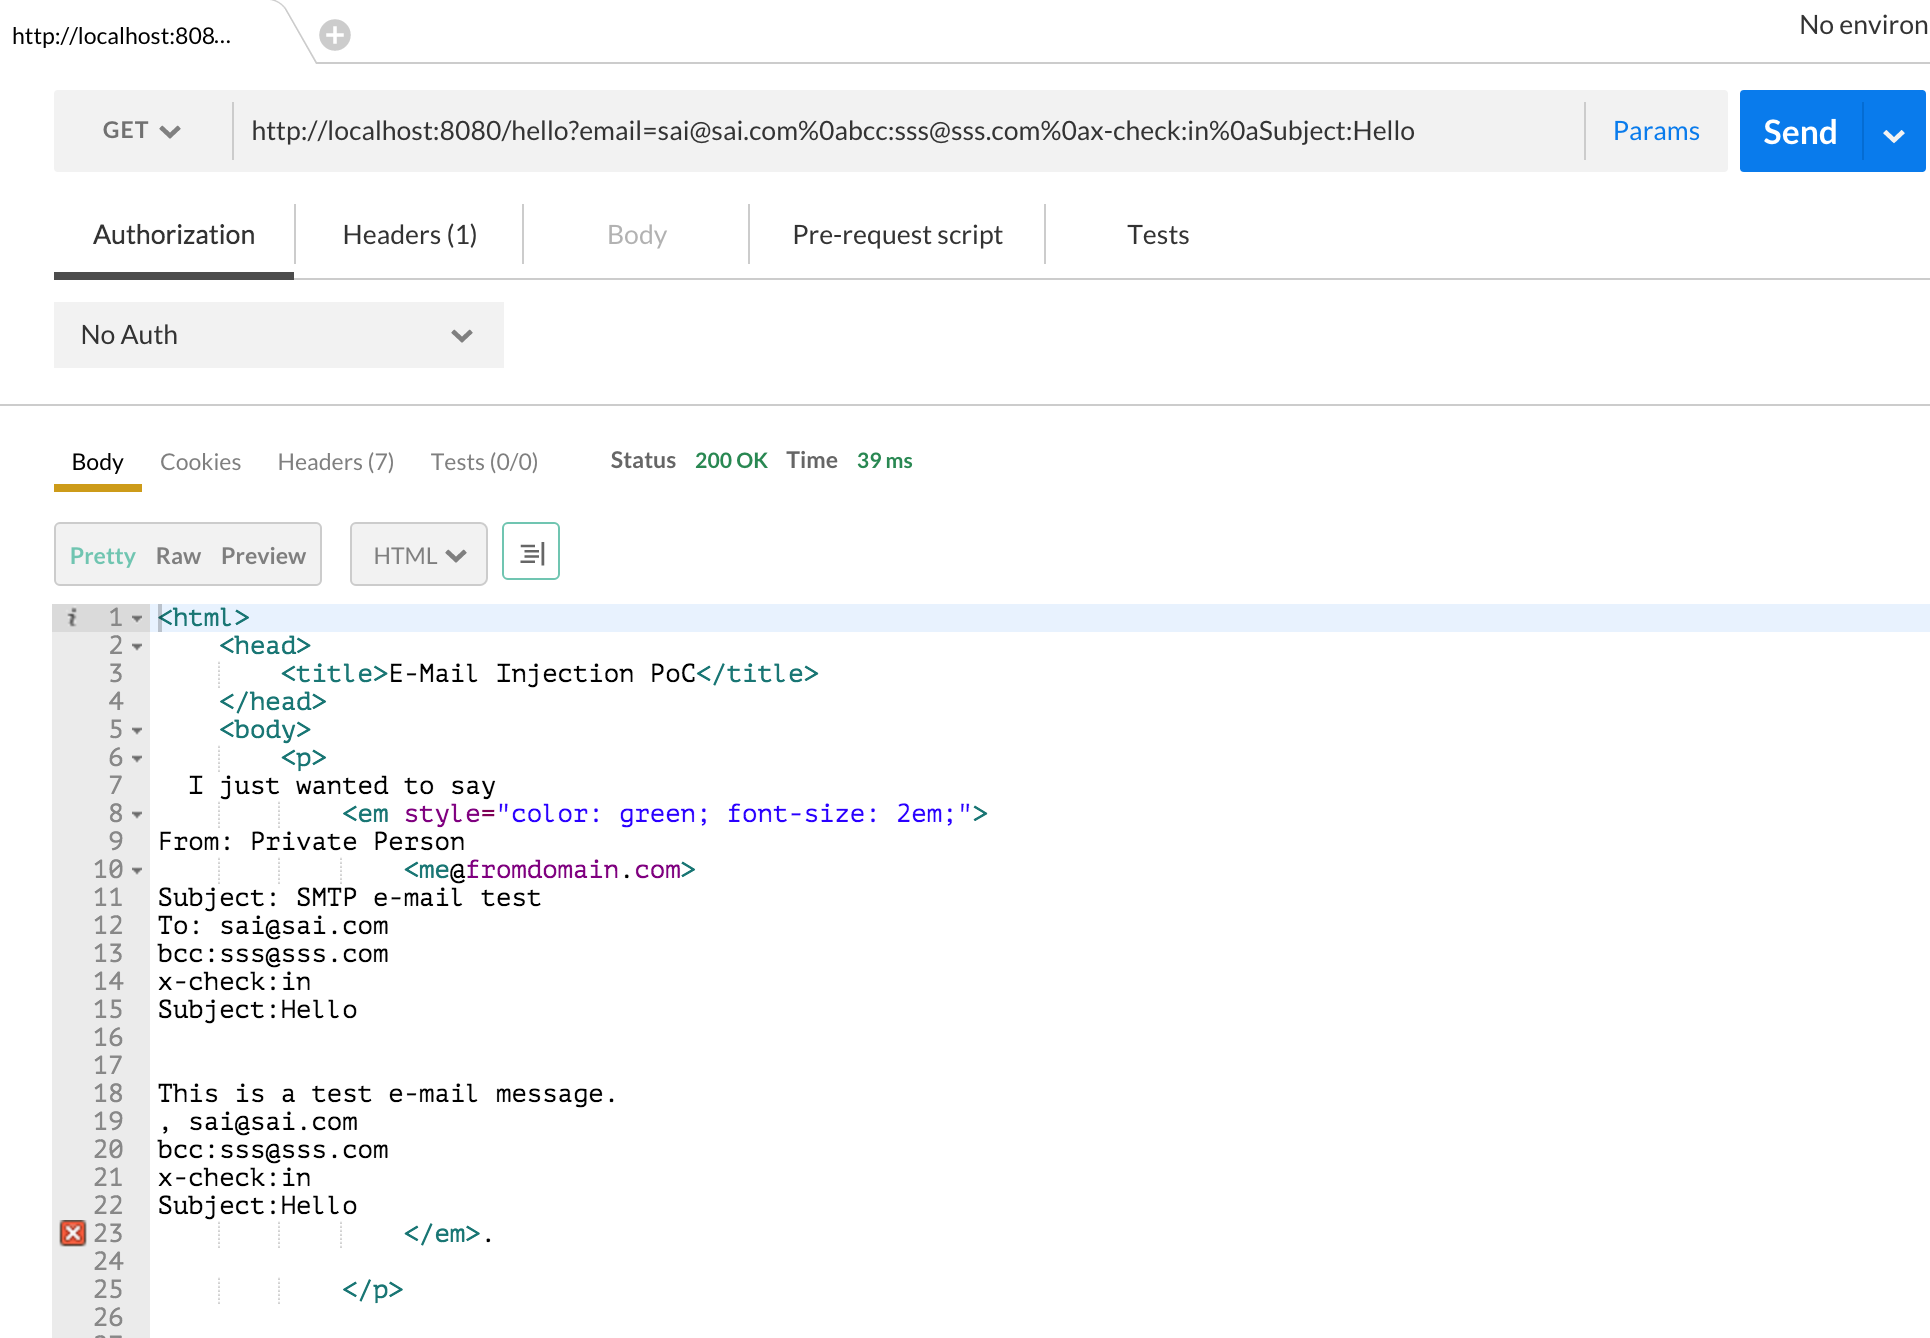
\includegraphics[width=14cm, height=8cm]{System/EMI_Postman_Ruby}
	\caption[\titlecap{Fuzzing a request for the Ruby backend}]{Fuzzing a request for the Ruby backend, the payload can be seen inside the address bar.}
	\label{fig:postmanruby}
\end{figure}

\begin{figure}[!htbp]
	\centering
	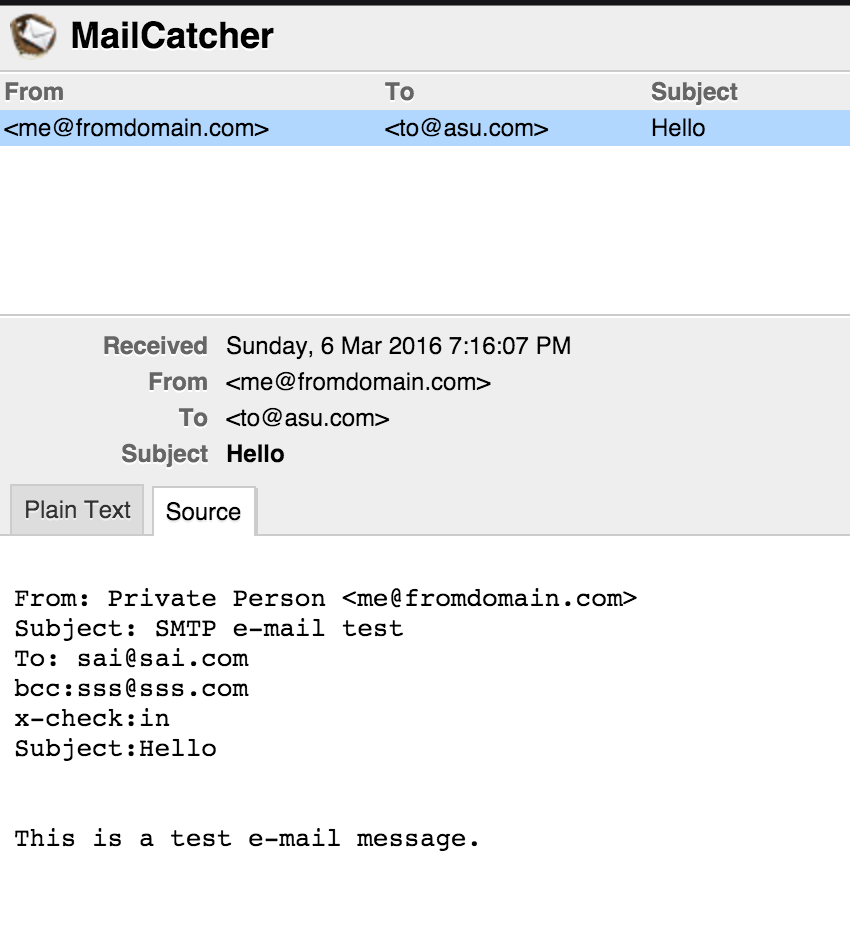
\includegraphics[width=14cm, height=8cm]{System/EMI_Mailcatcher_Ruby}
	\caption[\titlecap{E-Mail header injection proof of concept - Ruby}]{E-Mail header injection proof of concept - Ruby, we can see that multiple headers (bcc, x-check, subject) have been inserted into the resulting e-mail.}
	\label{fig:mailcatcherruby}
\end{figure}
	
	\section{Evaluation}

We ran our system on the web at large, attempting to discover \ehi vulnerabilities in web applications. 
\subsection{Collected Data}

From our extensive crawl of the web, we were able to gather the data
shown in Table~\ref{tab:data}. We ran the system for 76 days, during which our system crawled \urls unique URLs,
and found a total of \forms\ forms from \uniqueforms\ unique domains. Out of these forms, our system
found \emailforms\ forms that contained an \email field, from \uniqueemailforms\ unique domains.

\begin{table}[!htbp]
	\centering
	\begin{tabular}{|c|c|c|}
		\hline
		\multicolumn{1}{|c|}{\textbf{S.No}} &
		\multicolumn{1}{c|}{\textbf{Type of Data}} &
		\multicolumn{1}{c|}{\textbf{Quantity}}\\
		\hline
		1 & URLs Crawled & \urls \\
		\hline
		2 & Total Forms found & \forms \\
		\hline
		3 & Forms with E-Mail Fields & \emailforms \\
		\hline
	\end{tabular}
	\caption[\titlecap{Collected data}]{The data collected for our project.}
	\label{tab:data}
\end{table}


\subsection{Fuzzed data}
We performed our fuzzing attempts on the gathered data with both the regular payload and malicious payload. Table~\ref{tab:fuzzed_data} shows the quantity of e-mails that we received for each payload. We explain in detail what each piece of data shown in the table represents, in the following sections.
\begin{table}[tbp]
	\centering
	\scriptsize
	\begin{tabular}{|c|c|c|}
		\hline
		\multicolumn{1}{|c|}{\textbf{Type of fuzzing}} &
		\multicolumn{1}{c|}{\textbf{Forms fuzzed}} &
		\multicolumn{1}{c|}{\textbf{E-Mails received}}\\
		\hline
		Regular payload & \fuzzed & \recd \\
		\hline
		Malicious payload & \malfuzzed & \success \\
		\hline
	\end{tabular}
	\caption[\titlecap{Fuzzed data}]{The data that we fuzzed and the   e-mails that we received.}
    \vspace{-5ex}    
	\label{tab:fuzzed_data}
\end{table}

\paragraph{E-Mail received from forms}
The e-mails that we received can be broadly categorized into two categories:
\begin{enumerate}
	\item E-Mails due to regular payload\\
	This represents the total number of websites that sent e-mails to us. This indicates that we were able to successfully submit the forms on these sites.
	
	\item E-Mails due to malicious payload\\
    Once we receive an e-mail from a website due to the regular payload, we go back and fuzz those forms with more malicious payloads. This field, in essence, represents the total number of unique URLs that contain E-Mail Header Injection vulnerability.
\end{enumerate}




\subsection{Analysis of the Received \Email Data}
During our analysis of the received \emails, we found that the \emails that we received belonged to three categories:
\begin{enumerate}
	\item \Emails with the \texttt{bcc} header successfully injected\\
	  This form of injection was our initial objective, and we found
% Adam: Sai, why isn't this number a command? - DONE.
      \ehibcc such \emails in our received \emails. This validates that the web applications that sent these \emails are vulnerable to \ehi.
	
	\item \Emails with the \texttt{to} header successfully injected\\
	We discovered an unintended vulnerability class during our analysis, which we call \texttt{To~header injection}. These injections reflect the ability to inject any number of \email addresses into the \texttt{to} field of the SMTP message while being unable to inject any other header into the \emails. We found \ehito such \emails in our received \emails. We attribute this behavior to inconsistent sanitization by the application. 
    % Adam: I can't understand what this sentence is trying to say - Removed.
	
	While not allowing us complete control over content of the \emails sent, \texttt{To header injection} makes it possible to append any number of \email addresses, thereby enabling us to leak information or perform DoS (Denial of Service) attacks against the web application.
	
	\item \Emails with the \texttt{x-check} header successfully injected\\
    The third category of \emails received were \emails with the \texttt{x-check} header injected. As discussed in Section~\ref{analyze:detect_x_check}, 
    we can differentiate between unsuccessful attempts and successful attempts by injecting the additional header and checking whether headers other than the \texttt{bcc} header can be injected into the generated \email. \ehixcheck \emails were received with the \texttt{x-check} header injected.
\end{enumerate}

% Adam: Sai, we need to put the actual numbers in the text. We cannot count on the readers to look at the table (of course, we should use the commands
We list each category and the number of \emails received by that category in Table~\ref{tab:analysis}. 
We explain the combination of these header injections (4-7) as follows:

\begin{table}[tbp]
	\centering
	\scriptsize
	\begin{tabular}{|p{.32\textwidth}|p{.13\textwidth}|}
		\hline
		\textbf{Type of Injection} & \textbf{No. of e-mails received}\\
		\hline
		E-Mail Header Injections with \texttt{bcc} header & \ehibcc \\
		\hline
		E-Mail Header Injections with \texttt{x-check} header & \ehixcheck \\
		\hline
		\texttt{To header} injections alone & \ehito \\
		\hline
		Injections with both \texttt{bcc} and \texttt{x-check} headers & \ehibccxcheck \\
		\hline
		Both \texttt{To header} injections and x-check headers &
		\ehitoxcheck \\
		\hline
		\texttt{x-check} headers found in \texttt{nuser} e-mails & \ehinuserxcheck \\
		\hline
		Unique \texttt{x-check} headers found in \texttt{nuser} e-mails & \ehiuniquenuserxcheck \\
		\hline
		Total successful injections (1 + 3 + 7) & \success \\
		
		\hline
	\end{tabular}
	\caption[\titlecap{Analysis of the data}]{Classification of the e-mails that we received into broad categories of the vulnerability.}
	\label{tab:analysis}
\end{table}


\begin{itemize}
	\item \Email Header Injections with both \texttt{bcc} and \texttt{x-check} headers\\
	  These represent the scenario where an attacker can inject multiple headers into the \emails. We can see that 54\% of the received \texttt{bcc} header injected \emails are also susceptible to being injected with additional headers.
      % Adam: What is the exact percentage? We should use that rather than an approximate number - DONE.
	
	\item Both \texttt{To} header injections and \texttt{x-check} headers \\
	This combination shows us that in addition to being able to inject into the \texttt{To} fields, we injected additional headers into the \email. It is not clear what causes this behavior; however, these can be exploited to achieve the same result as a regular \ehi.
	
	\item Total \texttt{x-check} headers and unique \texttt{x-check} headers found in \texttt{nuser} \emails\\
		We found a total of \ehinuserxcheck \emails in the \texttt{nuser} account. Out of these, \ehiuniquenuserxcheck had unique form ids that were \emph{not} already found in the \texttt{maluser} account. We attribute these \emails to (probably) being sent by a web application that was built with Python or another language having a similar behavior with respect to ignoring duplicate headers while constructing an \email, thus appending the \texttt{x-check} header and \emph{not} the \texttt{bcc} header. 
      % Adam: What is the actual behavior? This is confusing. - Changed. DONE.
	
	\item Total successful injections\\
	  This represents the total number of successful injections. This includes the \ehi with \texttt{bcc} header\,(1), \texttt{To} header injections\,(3), and Unique \texttt{x-check} headers found in \texttt{nuser} \emails\,(7). A total of \success vulnerabilities were found by our system.

      % Adam: we need the actual #s here too. These are the core results of our analysis, they need to be in the text. - DONE.
	
\end{itemize}

\subsection[The Pipeline]{Understanding the Data Pipeline}
%This section serves to represent our pipeline quantitatively and graphically. 
Table~\ref{tab:pipeline} showcases the data gathered by our pipeline, with the differential changes at each stage of the pipeline. At each stage of the pipeline, the amount of data decreases, for instance, out of the \urls\ URLs we crawled, only \forms\ forms (\formsDelta) were found. Out of these, only \emailforms\ forms (\emailformsDelta) contained e-mail fields.

In our fuzzing attempts, the same behavior is observed. We fuzzed \fuzzed\ forms with the regular payload, which resulted in a total of \recd\ e-mails~(\recdDelta). After analysis of the received e-mails, we further fuzzed \malfuzzed\ forms, which resulted in \success\ e-mails (\successDelta) which contain the vulnerability across \ips IP addresses from \domains domains.

We attribute the difference in the number of forms found to the number of forms fuzzed (a difference of \diffFoundFuzz forms) to the presence of bot-blocking mechanisms on a website (discussed in Section~\ref{limitations}), though we do not know what percentage was caused by the individual bot-blocking mechanisms discussed in Section~\ref{limitations}. 

We would like to remark that over 1\% of the forms that were not fuzzed (100 out of \diffFoundFuzz) were also tested manually using PostMan to generate HTTP requests with payloads to verify that our system was working as intended.

\begin{table*}[tbp]
	\centering
	\normalsize
	\begin{tabular}{|l|c|c|}
		\hline
		\multicolumn{1}{|c|}{\textbf{Pipeline Stage}} &
		\multicolumn{1}{p{3cm}|}{\centering \textbf{Quantity}} &
		\multicolumn{1}{p{2.8cm}|}{\centering \textbf{Differential}
		$\Delta$ d2/d1 * 100}\\
		\hline
		Crawled URLs  & \urls &  --- \\
		\hline
		Forms found  & \forms & \formsDelta \\
		\hline
		E-Mail Forms found  & \emailforms & \emailformsDelta \\
		\hline
		Fuzzed with regular payload  & \fuzzed & \fuzzedDelta \\
		\hline
		Received e-mails  & \recd & \recdDelta \\
		\hline
		Fuzzed with malicious payload  & \malfuzzed & \malfuzzedDelta \\
		\hline
		Successful attacks  & \success & \successDelta \\
		\hline

	\end{tabular}
	\caption[\titlecap{Data gathered by our pipeline}]{Data gathered by our pipeline at each stage, with the differential between the stages.}
	\label{tab:pipeline}
\end{table*}



% Adam: this is an important part of our contribution, but I don't think that it belongs here. 
%% From our research, it is clear that E-Mail Header Injection is quite widespread as a vulnerability, appearing on \successDelta\ of forms that we were able to perform automated attacks on. This value acts as a lower bound for E-Mail Header Injection vulnerability, and can quite easily be much more if the attacks were of a more concentrated nature, crafted for the individual websites and less automated.

\subsection{Responsible Disclosure of Discovered Vulnerabilities}
After we discovered an \ehi vulnerability on a particular website, we attempted to notify the developers of the vulnerable web application, along with a brief description of the vulnerability.
We chose to \email the following mailboxes, following the rules specified in RFC~2142~\cite{rfc2142}:
\begin{itemize}
	\item \texttt{security@domain.com} - Security bulletins or queries.
	\item \texttt{admin@domain.com} - The administrator of a website.
	\item \texttt{webmaster@domain.com} - Synonym for administrator, same functionality as admin.
\end{itemize}
 
Out of the \domains\ vulnerable domains found, only \emailedDefaultmailbox websites had the mailboxes able to receive \emails. For the remaining domains, we used the \texttt{whois}~\cite{whois} data to find the contact details of the owner and then \emailed them. The number of emails we sent and the number of developer responses we received is shown in Table~\ref{tab:devresp}.

\begin{table}[tbp]
\centering
\normalsize
\begin{tabular}{|c|c|c|}
	\hline
	\multicolumn{1}{|p{2cm}}{\centering \textbf{Notified websites}} &
	\multicolumn{1}{|p{2cm}|}{\centering \textbf{Developer Responses}} &
	\multicolumn{1}{p{2cm}|}{\centering \textbf{Confirmed discoveries}}\\
	\hline
	\domains\ & \responses & \confirmed \\
	\hline
\end{tabular}
	\caption[\titlecap{}]{Responsible disclosure of the discovered vulnerabilities to developers and the number of received responses.}
	\label{tab:devresp}
\end{table}

% Adam: did we get updated notifications? - updated. DONE.
We received \responses developer responses, confirming \confirmed discovered vulnerabilities. Four of the developers fixed the vulnerability on their website.
% is this done? 1 additional email asking for more information, but no confirmation.
From our research, it is clear that \ehi is quite widespread as a vulnerability, appearing on \successDelta\ of forms that we were able to perform automated attacks on. This value acts as a \emph{lower bound} for prevalence of \ehi vulnerability, and can quite easily be larger if the attacks were broader, crafted for the individual web application, and  less automated. 

\subsection{Exploitation Evidence}
We compared the \ips IPs that our system found to be vulnerable to \ehi against 13 well-known IP blacklists, to see if these IPs were being exploited by attackers to send spam. The blacklists that we used were: 
\texttt{zen.spamhaus.org},
\texttt{spam.abuse.ch},
\texttt{cbl.abuseat.org},
\texttt{virbl.dnsbl.bit.nl},
\texttt{dnsbl.inps.de},
\texttt{ix.dnsbl.manitu.net},
\texttt{dnsbl.sorbs.net},
\texttt{bl.spamcannibal.org},
\texttt{bl.spamcop.net},
\texttt{dnsbl-1.uceprotect.net},
\texttt{dnsbl-2.uceprotect.net},
\texttt{dnsbl-3.uceprotect.net},
\texttt{db.wpbl.info}.

We found that \ipsblacklist of these IPs were blacklisted on at least one of the above blacklists for sending out spam, and \ipsblacklistmulti of them were found on multiple blacklists. We do not have enough data to make an observation about whether these attackers are exploiting \ehi to send out the spam, as an alternative hypothesis is that these IPs are on the blacklists because the server has different vulnerabilities that attackers exploit to cause the server to send spam (assuming that the server is normally benign).  

\subsection{Emails with Malicious Attachments}
We checked the \emails received by the `reguser' account (which are injected with regular \email addresses and not malicious data) for the presence of attachments that may contain malicious software, which will indicate that the server itself is not benign. 

To do this, we passed the \totalattachmentcount attachments we received to VirusTotal~\cite{virustotal} -- an online virus and malware scanner that checks for the presence of malware by running 40+ virus scanners on the uploaded files. We found that out of the \totalattachmentcount attachments, \totalvirusemails \emails contained malicious attachments, out of which \totalvirusattachmentcount were from unique domains. 
%It is to be noted that none of these domains were found on the spam analysis we did earlier, indicating that if these could be exploited, we could send emails with malicious attachments to other people using these servers.


	
	\section{Discussion}
    In this section, we discuss the lessons learned, the limitations of our system, and how to mitigate \ehi vulnerabilities.
\subsection{Lessons Learned}
    From our results, it is evident that the vulnerability exists in the wild. Despite its relatively low occurrence rate compared to the more popular SQL Injection and XSS (Cross-Site Scripting), when we take the total number of websites on the World Wide Web --- 1,018,863,952 according to Internet Live Stats \cite{InternetLiveStats2016} as of early 2016 --- and calculate \successDelta\ percent (the occurrence rate of E-Mail Header Injection vulnerability as found by our system) of that number, we end up with 11,309,390 websites - a pretty significant number. We agree that an extrapolation of that kind might not be an accurate measure of the prevalence of the vulnerability. However, even with as few as a thousand websites affected by this vulnerability, it can still have a disastrous impact on these websites, and also on overall World Wide Web due to the traffic caused by the sheer number of generated e-mails. 
    
    After analyzing the results, we would like to make a few more observations. We believe that one of the reasons for the small percentage of occurrence (compared to SQL Injection or XSS), can be attributed to what we like to call the `car parking analogy'.
    The car parking analogy is something like this: Imagine that we are parking a car on a road that is prone to attacks by thieves. Now, if all the cars were unlocked, the car that is most likely to get stolen is quite unsurprisingly the most expensive one or the one that is easiest to get away with.
    
    Now imagine the same thing on the World Wide Web: we have websites that can each have multiple vulnerabilities. Now, it makes sense for an attacker to try and attack websites with more widespread vulnerabilities such as SQL Injection or XSS, rather than attempt to exploit E-Mail Header Injection, seeing as this requires a more concentrated effort, with carefully crafted payloads and a waiting time for the e-mail to be delivered. SQL Injection attacks and XSS attacks are also better documented, with well-known attack vectors, and automated tools to help detect the presence of these vulnerabilities on websites.
    
    This also gives more incentive for the website developer to add protection against attacks such as SQL injection and XSS. The developer might then (possibly with the help of a sanitization library) sanitize the user input and remove \emph{all} special characters, including the newline characters (\textbackslash{}n, \textbackslash{}r), which adversely affects E-Mail Header Injection attacks.

	We come to this conclusion because of our discovery of the \dq{\texttt{To header injection}}. Clearly, this is possible due to incomplete sanitization performed by the application. We suspect that this incomplete sanitization is actually sanitization that is performed for some other vulnerability, and not specifically for E-Mail Header Injection attacks. We would also like to remark that \dq{\texttt{To header injection}} is not complete E-Mail Header Injection, but only a special subset.
	
    Thus, indirectly, this kind of protection against other attacks affects the attempts to perform E-Mail Header Injection. However, this does not completely negate the attempts if the checks are only on the client-side. Also, even with server-side validation, often, the only input fields that are validated are ones that are either inserted into the database (SQL Injection) and the ones that are displayed to the user as part of the web site (XSS).

	A second and a far more common reason for our fuzzing attempts to fail is the bot-blocking mechanisms built into the websites. CAPTCHAs (as explained in Section \ref{issues:captcha} and in the following section) pose a very difficult problem for our system to exploit E-Mail Header Injection, even if it is present.

	This does not mean that the vulnerability is not a large threat. In fact, this vulnerability can also have some major consequences, the least of which can be spamming and phishing attacks.
	In today's digital world, identity theft has become all the more common. E-Mail Header Injection provides attackers with the ability to easily extract information about users, not just from a server, but from the user himself, by sending him fake messages that look extremely authentic, since these messages are sent by the mail server of the website itself.
    
    From our research, we found two different forms of the E-Mail Header Injection Vulnerability: the first one is the traditional one, where we are able to inject any header into the forms, allowing us complete control over the contents of the e-mail. We identify this with the presence of both the \dq{\texttt{bcc}} header and the \dq{\texttt{x-check}} header. This is the most potent form of the vulnerability and is found on quite a few websites. This is also the vulnerability that is documented and discussed on many websites.
    
    The second attack is an interesting one, as this has not yet been documented, and provides the ability to inject multiple e-mail addresses into only the \dq{\texttt{To}} field. We christened this as \dq{\texttt{To header injection}}. In this form of the vulnerability, we are able to simply add addresses to the \dq{\texttt{To}} field of the form with newlines separating the e-mail addresses. Whether this particular form of the vulnerability is found due to the websites in question, or whether this is an implementation issue with a particular language or framework, is unclear. However, from our preliminary analysis, it is evident that these websites do not share much with respect to the languages and frameworks used. 
    Even in this form of the attack, we are still able to extract information that should be private to a given user, and in some of these cases, able to inject enough data to spoof the first few lines of the e-mail message. From Table~\ref{tab:analysis}, information leakage using \dq{\texttt{To header injection}} was possible on 142 forms, while spoofing using \dq{\texttt{To header injection}} was possible on 11 forms.
    
    While not being as impactful as the primary vulnerability, this second form of the vulnerability does still provide the ability to send e-mails to multiple recipients, and can easily result in information leakage or spam generation on a large scale.
    

\subsection[Limitations]{Limitations of the Project}
\label{limitations}
	This section complements Section \ref{sys:issues}, and discusses the limitations of our project. The following list, although not exhaustive, goes into the limitations of our project in detail: 
	\begin{itemize}
		\item CAPTCHAs - As noted in section \ref*{issues:captcha}, CAPTCHAs pose a significant problem to our automated system. As CAPTCHAs are designed to be robust, there is no easy way to break them. There has been considerable research in this area~\cite{captchas2}, \cite{captchas} to name a few and although not impossible to break, it remains out of the scope of this project, and thus, we chose to ignore websites which require CAPTCHA verification.
		\item JavaScript Apps - Due to the growing emphasis on responsive web applications, more and more single-page web applications are being built purely with JavaScript. Even conventional applications are now making use of JavaScript to dynamically insert content and update the pages. This means that these dynamically injected components are not a part of the initial source code that is sent to the client by the web server.
		
		Thus, our system never receives dynamically injected forms from the web server and hence is unable to detect whether these vulnerabilities are present in such forms. The only workaround would be, to use a JavaScript engine to query for the \lstinline|document.getElementsByTagName('html')[0].innerHTML| (from inside web browser automation tools like Selenium, etc.), and then use that as the source code for our URL.
		
		Since this would add unnecessary bulk and complexity to our application, we chose not to do it, and thus, we consider this to be a limitation.
		
		\item Blogs powered by WordPress/Drupal\\
        In addition to what was discussed in Section \ref{issues:cms}, we found that certain WordPress plugins also prevent the E-Mail Header Injection attack by sanitizing user input on Contact Forms. Some of these plugins are discussed in the following section. Although not all websites built with WordPress are secure from the attack, between the presence of the plugins on some websites, and getting tagged as `spambots' by others, we were able to do vulnerability analysis on very few sites powered by WordPress.
		
		\item Blacklisting by websites and ISPs\\
        During the actual crawl, our system was blacklisted by a few websites (mostly WordPress ones), and Internet Service Providers (ISPs). We then created a blacklist of our own to ensure that we did not inject these websites. The result was that we could not gather any data about these websites.
		
		\item E-Mail libraries\\
        E-Mail libraries like the PHP Extension and Application Repository's (PEAR) mail library provide sanitization checks for user input. While this is technically not a limitation of our project, it still makes it such that we are not able to inject these sites successfully.
        A few other libraries for each language are discussed in the following section.
        
        \item Websites that are not in English\\
        Because we are only searching for the words \texttt{e-mail}, \texttt{mail} or \texttt{email} within the form, if the website does not use English names for its forms, our system will not be able to find the presence of an e-mail field. An example is shown in Listing~\ref{code:htmlfrench}. Here, the French word for \texttt{e-mail} --- courrier électronique --- is used, and our system is unable to find the presence of the e-mail form.
	\end{itemize}
	
\lstset{language=HTML,caption={HTML page with e-mail form, written in a different language - French.},label={code:htmlfrench}, literate=%
	{é}{{\'e}}1}
\begin{lstlisting}
<!doctype html>
<html lang="fr">
<head>
<meta charset="utf-8">
<meta name="author" content="Sai Pc">
<title>Mock Email</title></head>
<body>
<form action="{Replace with path to back-end}" method="post">
<input type="text" placeholder="courrier électronique" 
	name="courrier_électronique"><br>
<textarea name="msg" rows="20" cols="120"></textarea>
<input type="submit" value="courrier électronique!">
</form></body>
</html>
\end{lstlisting}

\subsection{Assumptions}
In addition to the limitations that were already discussed, we made certain assumptions while building the system. This section describes the assumptions and explores to what extent these hold true:
\begin{enumerate}
	\item \textbf{Crawler is not blocked by firewalls}\\
	This is a requisite for our system to work. If the Crawler is blocked for any reason, we do not get the data feed for our system, and without this input, it is almost impossible to set our system up.
	
	\item \textbf{The Crawler feed is an ideal representation of the World Wide Web} \\
	This is a reasonable expectation, albeit an unrealistic one.
	
	It is unrealistic because Crawlers work on the concept of proximity. They detect for the presence of In-Links and Out-Links from a particular URL, and hence the returned URLs are usually related to each other (at least the ones that are returned adjacent to each other).
	
	However, this assumption is reasonable due to the `Law of averages' \cite{wiki:Law_of_averages}, the `Law of big numbers' \cite{wiki:Law_of_large_numbers}, and the concept of `Regression to the mean' \cite{wiki:Regression_toward_the_mean}. Simply stated, a crawl of this large magnitude should give us a very distributed sample of the overall Web, eventually converging to the average of all websites in existence.
	
	\item \textbf{Injection of \texttt{bcc} indicates the existence of E-Mail Header Injection Vulnerability} \\
	We assume that the ability to inject a \texttt{bcc} header field is proof that the E-Mail Header Injection vulnerability exists in the application. We do not inject any additional payloads that can modify the subject, message body, etc.\ as this analysis is designed to be as benign as possible.
	We believe that this is a reasonable assumption, as altering e-mail headers is a goal of exploiting E-Mail Header Injection vulnerability.
\end{enumerate}

That concludes our discussion about the design of the system. To recap, we discussed our approach, the system architecture and how the components fit into our architecture. We also discussed the issues faced, and the assumptions that we made while building the system. %The next section describes, in brief, the experimental setup we used for our system.
\subsection{Ethics}

To make sure that our system did not cause any harm to the web applications that we crawled, we made sure that we did not inject any special characters other than the newline character% (characters that a developer would assume an average user could put in)
. We also had an informational website at the IP that we crawled from that described what \ehi was, and contained our contact details in case the developers of the web applications we crawled wanted to contact us. We maintained a separate blacklist of domain names that the owners did not want us to crawl, and ensured that our system did not crawl their domains.

\subsection[Mitigation Strategy]{How to prevent this attack}
\label{disc:mitigation}
This section describes the most common measures that can be taken to prevent the occurrence of this vulnerability, or at least reduce the impact.
\begin{itemize}
	\item Use Mail Libraries\\
	This is the preferred way of combating this vulnerability. Using a library that is well tested can remove the burden of input sanitization from the developer. Also, since most of these libraries are open-source, bugs are identified quicker and fixes are readily available.
	A list of known secure libraries for each popular language and framework is shown in Table~\ref{tab:maillib}.
	
	Using libraries such as PEAR Mail, PHPMailer, Apache Commons E-Mail, Contact Form 7, and Swiftmailer can significantly reduce the occurrence of E-Mail Header Injection vulnerability.
	\begin{table}[!htbp]
		\centering
		\begin{tabular}{|l|l|}
			\hline
			\multicolumn{1}{|c|}{\textbf{Language}} &
			\multicolumn{1}{c|}{\textbf{Mail Libraries}} \\
			\hline
			PHP & {{PEAR Mail\tablefootnote{PEAR Mail Website: https://pear.php.net/package/Mail}, PHPMailer\tablefootnote{PHPMailer Website: https://github.com/PHPMailer/PHPMailer}, Swiftmailer\tablefootnote{Swiftmailer Website: http://swiftmailer.org/}}}\\
			\hline
			Python & SMTPLib with email.header.Header\tablefootnote{instead of using email.parser.Parser to parse the header}\\
			\hline
			Java & Apache Commons E-Mail\tablefootnote{Apache Commons E-Mail: https://commons.apache.org/proper/commons-email/}\\
			\hline
			Ruby & Ruby Mail \textgreater{}= 2.6\tablefootnote{Ruby Mail Website: https://rubygems.org/gems/mail}\\
			\hline
			WordPress & Contact Form 7\tablefootnote{Contact Form 7 Download: https://wordpress.org/plugins/contact-form-7/}\\
			\hline
		\end{tabular}
		\caption[\titlecap{Mail libraries that prevent e-mail header injection}]{Mail libraries that prevent e-mail header injection.}
		\label{tab:maillib}
	\end{table}
	% changes to be made amrked in sublime
	\item Use a Content Management System (CMS) \\
	Content management systems like WordPress and Drupal include certain libraries and plugins to prevent E-Mail Header Injection. Thus, websites built with such CMS' are usually resistant to these attacks. However, it is advised to use the right E-Mail plugins when using such CMS', as not all plugins might be secure.
	An example of a secure plug-in is included as part of Table~\ref{tab:maillib}.
	
	\item Input Validation\\
	If neither of the two options above is feasible, due to reasons such as the website being an in-house production, or due to lack of support infrastructure, developers can choose to perform proper input sanitization. Sanitization should be done keeping in mind RFC5322 \cite{rfc5322}, and care must be taken to ensure that all edge cases are taken into account.
	
	Client Side validation alone is not sufficient, and must be supplemented by server-side validation to mitigate the attack. Constant updates to validation methods are required so that new attack vectors do not harm the website in any way.
	Test driven development for such validation methods is also encouraged so that we can be reasonably sure of our defense mechanisms.
\end{itemize}


	
	\section{Related Work}

% Adam: Sai, can you combine all the \cites at the same line like I did for the others? 
There are different approaches to finding vulnerabilities in web applications, and most approaches will be either Black-Box testing or White-Box testing.
Our work is based on the black-box testing approach to finding vulnerabilities on websites, and research has made use of this methodology to find vulnerabilities in web applications~\cite{Beizer:1995:BTT:202699, Huang, kals2006secubat, payet13:ears-in-the-wild, zanero2005automatic}. There has been significant discussion on both the benefits of such an approach~\cite{black-box} and its shortcomings~\cite{Doupe2012, Doupe2010}.

Our work does not intend to act as a vulnerability scanner, but as a means to identify an \ehi vulnerability in a given web application. In this sense, because we are injecting payloads into the web application, our work is related to other injection based attacks, such as SQL Injection~\cite{sql1, sql0, sql2}, Cross-Site Scripting \cite{Injection1, KleinAmit}, HTTP Header Injection~\cite{sessionride}, and the related Simple Mail Transfer Protocol (SMTP) Injection~\cite{Terada2015}.

The attack described by Terada~\cite{Terada2015} is one that attacks the underlying SMTP mail servers by injecting SMTP commands (which are closely related to E-Mail Headers and usually have a one-to-one mapping, e.g., \texttt{To} e-mail header has a corresponding \texttt{To} SMTP header) to exploit the SMTP server's pipelining mechanism. Terada also describes proof-of-concept attacks against certain mailing libraries such as \texttt{Ruby Mail} and \texttt{JavaMail}. This attack, although trying to achieve a similar result, is distinctly different from ours. The paper makes this observation and discusses why it is different from \ehi.

In comparison, our work tries to exploit application-level flaws in user input sanitization, which allow us to perform this attack. Our work does not intend to exploit the pipelining mechanism, but to exploit the implementation of the mail function in most popular programming languages, which leaves them with no way to distinguish between user supplied headers and headers that are legitimately added by the application.

Although \ehi vulnerabilities have been present for over a decade, there has not been much written about it in the literature, and we find only a few articles on the Internet describing the attack.

The first documented article dates to over a decade ago; a late 2004 article on phpsecure.info~\cite{Tobozo} accredited to user \lstinline|tobozo| describing how this vulnerability existed in the reference implementation of the mail function in PHP, and how it can be exploited. Following this, we found other blog posts~\cite{Calin, DK, Injection2, Nicol, Pope}, each describing how to exploit the vulnerability by using newlines to camouflage headers inside user input. A wiki entry~\cite{Injection} also describes the ways to prevent such an attack. However, none of these articles have performed these attacks against real-life websites.

Another blog post written by user \lstinline|Voxel@Night|~\cite{Tendencies2014}, recounts an actual attack against a WordPress plugin, \texttt{Contact Form}, with a proof of concept\footnotemark. It also showcases the vulnerable code in the plugin that causes the vulnerability. However, this article targets just one plugin and does not aim to find the prevalence of said plugin usage. Neither does it inform the creators of the plugin to fix the discovered vulnerability.
\footnotetext{Note that this plugin is used actively on 300,000 websites (according to~\cite{BestWebSoft2016}), but is yet to be fixed.}
The vulnerability was described briefly by Stuttard and Pinto in their book, ``\emph{The Web Application Hacker's Handbook: Discovering and Exploiting Security Flaws}''~\cite{stuttard2011web}. The book, however, does not go into detail on either the attack or the ways to mitigate such an attack. Our work, on the other hand discusses the means to mitigate the attack. We also describe, in detail, the payloads that can be used and the need for varying the payloads (Section~\ref{Comp:Fuzzer}).

To the best of our knowledge, no other research has been conducted to determine the prevalence of this vulnerability across the World Wide Web. We have managed to, on a large scale, crawl and inject web applications with comparatively benign payloads (such as the BCC header) to identify the existence of this vulnerability without causing any ostensible harm to the website. Our injected payloads \emph{do not contain any special characters other than the newline character} and thus cannot cause any unintended consequences. Also, because we are only injecting a payload with the \texttt{bcc} header, the underlying mail servers should not be affected by the additional load. Our work serves to not only prove the existence of the vulnerability on the World Wide Web but to quantify the prevalence.

	
	\chapter{Conclusion}
We have showcased a novel approach involving black-box testing to identify the presence of E-Mail Header Injection in a web application. Using this approach, we have demonstrated that our system was able to crawl \urls\ web pages finding \forms\ forms, out of which \emailforms\ forms were fuzzable. We fuzzed \fuzzed\ forms and found \recd\  forms that allowed us to send/receive e-mails. Out of these, we were able to inject malicious payloads into \malfuzzed\ forms, identifying \success\ vulnerable forms (\successDelta\ success rate). This indicates that the vulnerability is widespread, and needs attention from both web application developers and library makers. 

We hope that our work sheds light on the prevalence of this vulnerability and that it ensures that the implementation of the `mail' function in popular languages is fixed to differentiate between User-supplied headers, and headers that are legitimately added by the application, and that the RFC's are updated to be more stringent and make it less ambiguous for future implementations. 
	
	%
	% The following two commands are all you need in the
	% initial runs of your .tex file to
	% produce the bibliography for the citations in your paper.
	\bibliographystyle{abbrv}
	\bibliography{biblio}  
	% You must have a proper ".bib" file
	%  and remember to run:
	% latex bibtex latex latex
	% to resolve all references
	%
	%\balancecolumns
\end{document}
